\chapter{余切丛上的\personFloer{}同调}
\label{ch:cotangent-floer}

\stfhIndex{I038}{Anuoerdecaixiang}{阿诺尔德猜想（Arnol'd's conjecture）}
\stfhIndex{I046}{Fenduancedixianbijin}{分段测地线逼近（broken geodesic approximation）}
\stfhIndex{I053}{Shapulong}{沙普隆（Chaperon）}
\stfhIndex{I063}{Kangli-Zengdeer}{康利--曾德尔（Conley--Zehnder）}
\stfhIndex{I096}{Shengchenghanshu}{生成函数（generating function）}
\stfhIndex{I118}{Luodangbake-Xikelafu}{洛当巴克--西科拉夫（Laudenbach--Sikorav）}
20 世纪 60 年代，\personArnold{}首先在 (Ar65) 中预言了（余切丛上）\emph{\termLagrangianIntersectionTheory{}}的存在，并把它看作\personMorse{}理论的交点理论版本。他还提出了\emph{\personArnold{}猜想}：若 $N$ 是紧流形，则 $T^*N$ 的\termZeroSection{}之\termGeometricIntersectionNumber{}不小于 $N$ 上由\personMorse{}理论给出的临界点数。由于对后一个\personMorse{}理论不变量尚缺乏理解，该猜想的这个原始版本仍未解决。不过，\personHofer{} (H85) 用作用量泛函经典变分理论的\emph{直接方法}证明了它的上同调版本。这一工作受到\personConley{}和\personZehnder{}更早证明 (CZ83) 的启发；他们所证的是关于\termHamiltonianDiffeomorphism{}不动点数的\personArnold{}猜想。大致在同一时期，\personMarcChaperon{} (Ch84) 以及\personLaudenbach{}和\personSikorav{} (LS85) 在证明同一结论时，采用了作用量泛函的\emph{\termBrokenGeodesicApproximation{}}和\emph{生成函数}方法。这以简单的、多少算是标准的\personMorse{}理论，取代了\personHofer{}证明中复杂的分析技术细节。

\personChaperon{}以及\personLaudenbach{}和\personSikorav{}发表的证明使人联想到\personConley{}和\personZehnder{}的证明 (CZ83)，因为两种证明都把无限维问题化为有限维问题。（\personLaudenbach{}和\personSikorav{}的生成函数方法后来由\personSikorav{} (Sik87) 进一步发展，并最终发展成\personViterbo{}的在无穷远处二次的\emph{生成函数}理论 (Vi92)。）

\stfhIndex{I080}{Fuluoer}{弗洛尔（Floer）}
\stfhSubIndex{I087}{Fuluoertongdiao}{弗洛尔同调（Floer homology）}{Zaiyuqiecongshang}{在余切丛上（on cotangent bundles）}
与此同时，\personFloer{}在 (Fl88b) 中引入了一种一般的无限维同调理论，如今称为\termFloerHomology{}。该理论以研究某个\termCauchyRiemannType{}椭圆方程的\termModuliSpace{}为基础；这个方程作为与所论变分问题相伴的\termActionIntegral{}的\termLtwoGradientFlow{}出现。特别地，如果我们在余切丛中取
\[
  L_0=\phi(o_N),\qquad L_1=o_N,
\]
那么上述\personHofer{}定理是\personFloer{} (Fl88a) 的一个特例（至少在不计定向问题时如此；该问题后来在 (Oh97b) 中得到了解决）。（\personFloer{}的构造不仅适用于辛几何中的作用量泛函，也适用于低维拓扑中出现的各种一阶椭圆系统，例如\termAntiSelfDualYangMillsEquation{}和\termSeibergWittenMonopoleEquation{}；它已成为近期低维拓扑与辛拓扑发展中的一项基础性工具。）

\stfhIndex{I055}{Jingdianzuoyongliangfanhan}{经典作用量泛函（classical action functional）}
\stfhIndex{I194}{Weitaibobubianliang}{维泰博不变量（Viterbo's invariants）}
在 (Oh97b) 中，本书作者利用了与经典作用量泛函相伴的\termFloerComplex{}中固有的自然\termFiltration{}，给出了\personViterbo{}不变量的一个\personFloer{}理论构造。这一构造的部分动机来自\personWeinstein{}的如下观察：经典作用量泛函
\[
  \mathcal A_H(\gamma)
  =\int_\gamma p\,dq-\int_0^1 H(t,\gamma(t))\,dt
\]
是\termLagrangianSubmanifold{} $\phi_H^1(L)$ 的一个典范“生成函数”。

本章简要总结余切丛上的\personFloer{}理论。在这里，我们可以展示\termFloerHomology{}在辛拓扑中已知应用的几乎所有方面，而无需研究\termBubblingPhenomenon{}，因为余切丛上不会发生冒泡。我们把这一至关重要的\termBubblingPhenomenon{}及其在一般情形下的技术基础，留到后续各章再加研究。

\section{作为生成函数的作用量泛函}
\label{sec:action-functional-generating-function}

我们先把第一变分公式 (3.4.15) 限制到余切丛的情形。此时 $\alpha=-\theta$，而\personLiouville{} 1-形式为 $\theta=\sum_{i=1}^n p_i\,dq^i$，于是
\begin{equation}
\begin{split}
  d\mathcal A_H(\gamma)\xi
  ={}&\int_0^1\omega_0\bigl(\dot\gamma(t)-X_H(t,\gamma(t)),\xi(t)\bigr)\,dt
      +\bigl\langle\theta(\gamma(1)),\xi(1)\bigr\rangle \\
     &-\bigl\langle\theta(\gamma(0)),\xi(0)\bigr\rangle .
\end{split}
\label{eq:cotangent-action-first-variation}
\end{equation}
这里 $\gamma:[0,1]\to T^*N$，而 $\xi\in\Gamma(\gamma^*T(T^*N))$ 是沿 $\gamma$ 的一个向量场。

对这个公式稍加思考，就会得到若干重要结论。

首先，我们考虑始于\termZeroSection{}中某一点的道路 $\gamma:[0,1]\to T^*N$。记
\[
  \Omega(0;o_N)=\{\gamma\mid\gamma(0)\in o_N\}.
\]
有一个自然映射
\[
  \pi\operatorname{ev}_1:\Omega(0;o_N)\longrightarrow N,
\]
它由
\begin{equation}
  \pi\circ\operatorname{ev}_1(\gamma)=\pi(\gamma(1))
  \label{eq:projection-evaluation}
\end{equation}
定义。这给出了 $\Omega(0;o_N)$ 在 $N$ 上的一个纤维化，它在 $q\in N$ 上的纤维为
\[
  \Omega(o_N,T_q^*N)
  =\{\gamma\mid\gamma(0)\in o_N,\ \gamma(1)\in T_q^*N\}.
\]
\stfhIndex{I078}{Xianweidaoshu}{纤维导数（fiber derivative）}
$\mathcal A_H$ 相对于 $\pi\operatorname{ev}_1$ 在 $q$ 处的纤维导数，无非是
\[
  \mathcal A_H:\Omega(o_N,T_q^*N)\longrightarrow\mathbb R
\]
的第一变分。因而
\[
  d^{\mathrm{fiber}}\mathcal A_H(\gamma)(\xi)
  =\int_0^1\omega_0\bigl(\dot\gamma(t)-X_H(t,\gamma(t)),\xi(t)\bigr)\,dt
\]
\stfhIndex{I019}{00-sigma-ah}{$\Sigma_{\mathcal A_H}$}
\stfhIndex{I077}{Xianweilinjieji}{纤维临界集（fiber critical set）}
对所有 $\xi\in T_\gamma\Omega(o_N,T_q^*N)$ 成立。因此，相应的\termFiberCriticalSet{}（记为 $\Sigma_{\mathcal A_H}\subset\Omega(0;o_N)$）由\personHamilton{}方程的解组成：
\[
  \dot x=X_H(t,x),\qquad x(0)\in o_N,\quad x(1)\in T_q^*N.
\]
由式~\eqref{eq:cotangent-action-first-variation}，注意在 $\Sigma_{\mathcal A_H}$ 上有
\[
  d\mathcal A_H(\gamma)(\xi)
  =\bigl\langle\gamma(1),d\pi(\xi(1))\bigr\rangle.
\]

\begin{exercise}
\label{ex:push-forward-action-one-form}
补全一个形式的启发式论证，由这个公式推出：1-形式 $d\mathcal A_H(\gamma)$ 的\termPushForward{}无非是 $\gamma(1)\in T_q^*N$。
\end{exercise}

\stfhIndex{I197}{Wensitan}{温斯坦（Weinstein）}
这就完成了下述命题的启发式证明。该命题是\personWeinstein{}观察到的。

\begin{proposition}[\personWeinstein{}]
\label{prop:action-functional-generates-image-zero-section}
在上述意义下，二元组 $(\mathcal A_H,\Omega(0;o_N))$ 是 $\phi_H^1(o_N)$ 的一个生成函数。
\end{proposition}

事实上，这个生成函数有一个自然的\termFiniteDimensionalReduction{}。我们称它为 $L_H=\phi_H^1(o_N)$ 的\termBasicGeneratingFunction{}，并记为 $h_H:L_H\to\mathbb R$。对给定的 $x\in L_H$，记
\[
  z_x^H(t)=\phi_H^t\bigl((\phi_H^1)^{-1}(x)\bigr).
\]
它是一条\termHamiltonianTrajectory{}，且依定义满足
\begin{equation}
  z_x^H(0)\in o_N,\qquad z_x^H(1)=x.
  \label{eq:basic-hamiltonian-trajectory-endpoints}
\end{equation}
我们回顾 (Oh97b) 中用到的如下基本引理，其证明留作习题。

\begin{lemma}
\label{lem:basic-generating-function}
定义函数 $h_H:L_H\to\mathbb R$ 为
\[
  h_H(x)=\mathcal A_H(z_x^H),
  \qquad
  z_x^H(t)=\phi_H^t\bigl((\phi_H^1)^{-1}(x)\bigr).
\]
则它满足
\[
  i_H^*\theta=dh_H.
\]
也就是说，$h_H$ 是 $L_H$ 的一个生成函数。我们称 $h_H$ 为 $L_H$ 的\termBasicGeneratingFunction{}。
\end{lemma}

\begin{exercise}
\label{ex:prove-basic-generating-function}
证明这个引理。
\end{exercise}

公式~\eqref{eq:cotangent-action-first-variation} 的另一个结论，是它刻画了 $\mathcal A_H$ 的变分理论中的\termNaturalBoundaryCondition{}。一个显然的\termNaturalBoundaryCondition{}是周期边界条件 $\gamma(0)=\gamma(1)$。下面给出一类更有趣的\termNaturalBoundaryCondition{}。

\begin{proposition}
\label{prop:tautological-form-vanishes-on-conormal}
对子流形 $S\subset N$，考虑余法丛 $i_S:\nu^*S\hookrightarrow T^*N$。则 $i_S^*\theta=0$。
\end{proposition}

\begin{proof}
取 $\xi\in T_\alpha(\nu^*S)$，并设 $\pi(\alpha)=x$。\footnote{译者注：原书此处写作 $\xi\in T_\alpha(T^*N)$，但依 $i_S^*\theta$ 的定义及下一句，应为 $\xi\in T_\alpha(\nu^*S)$；紧随其后的公式还脱漏了最外层右括号。译文据此补正。}我们有
\[
  i_S^*\theta(\xi)=\alpha(x)\bigl(d\pi(\xi(\alpha))\bigr).
\]
但这个配对为零，因为依定义有 $d\pi(\xi(\alpha))\in T_xS$ 和 $\alpha(x)\in\nu_x^*S$。证明完毕。
\end{proof}

由该命题，若把作用量泛函 $\mathcal A_H$ 限制到子集
\[
  \Omega_{S_0S_1}
  =\Omega(\nu^*S_0,\nu^*S_1)
  =\{\gamma:[0,1]\to T^*N
      \mid\gamma(0)\in\nu^*S_0,\ \gamma(1)\in\nu^*S_1\},
\]
则 $\mathcal A_H$ 的第一变分 $d\mathcal A_H$ 化为
\begin{equation}
  d\mathcal A_H(\gamma)(\xi)
  =\int_0^1\omega_0\bigl(\dot\gamma(t)-X_H(t,\gamma(t)),\xi(t)\bigr)\,dt.
  \label{eq:conormal-action-first-variation}
\end{equation}
我们指出，上面定义的道路空间 $\Omega(o_N,T_q^*N)$ 是余法边界条件的一个特例，它对应于 $S_0=N$ 和 $S_1=\{q\}$。

\cref{prop:tautological-form-vanishes-on-conormal}的一个立即推论是对临界点方程的如下刻画：$d\mathcal A_H|_{\Omega(S_0,S_1)}(\gamma)=0$ 当且仅当 $\gamma$ 满足
\begin{equation}
  \dot\gamma=X_H(t,\gamma(t)),
  \qquad
  \gamma(0)\in\nu^*S_0,\quad \gamma(1)\in\nu^*S_1.
  \label{eq:conormal-hamilton-equation}
\end{equation}

\begin{definition}[作用谱]
\label{def:conormal-action-spectrum}
我们把 $\operatorname{Spec}(H;S_0,S_1)$ 定义为临界值的集合，并称它为 $\mathcal A_H$ 在 $\Omega_{S_0S_1}$ 上的\termActionSpectrum{}，即
\[
  \operatorname{Spec}(H;S_0,S_1)
  =\{\mathcal A_H(z)\mid
      \dot z=X_H(t,z(t)),\ z(0)\in\nu^*S_0,\ z(1)\in\nu^*S_1\}.
\]
\end{definition}

\begin{proposition}
\label{prop:conormal-action-spectrum-measure-zero}
子集 $\operatorname{Spec}(H;S_0,S_1)\subset\mathbb R$ 是紧的，且测度为零。
\end{proposition}

\begin{proof}
如第 3.1 节所示，式~\eqref{eq:conormal-hamilton-equation} 的解与交集
\[
  \phi_H^1(\nu^*S_0)\cap\nu^*S_1
\]
之间存在一一对应。显然，这个集合是紧的。\footnote{译者注：原书在没有附加横截性或紧性假设时断言该交集“显然”紧；例如取 $H=0$ 且 $S_0=S_1=\{q\}$，该交集就是非紧的余切纤维 $T_q^*N$。因此原书此处的紧性论证不能按所写成立。}另一方面，从 $\nu^*S_1$ 到 $\mathbb R$ 的函数
\[
  h:x\longmapsto z_x^H\longmapsto\mathcal A_H(z_x^H)
\]
是光滑的，因而它在 $\phi_H^1(\nu^*S_0)\cap\nu^*S_1$ 上的像是紧的。\footnote{译者注：此前的 $z_x^H$ 与 $h_H$ 是针对 $x\in\phi_H^1(o_N)$ 定义的；此处却在一般 $S_0$ 下把 $h$ 写成 $\nu^*S_1$ 上的函数，并在下述习题中把其临界点集等同于 $\phi_H^1(\nu^*S_0)\cap\nu^*S_1$。原书没有给出完成这一推广所需的新定义或论证。}

\begin{exercise}
\label{ex:critical-points-basic-function}
$h$ 的临界点集与交集 $\phi_H^1(\nu^*S_0)\cap\nu^*S_1$ 重合，而 $h$ 的临界值集与 $\operatorname{Spec}(H;S_0,S_1)$ 重合。
\end{exercise}

把\personSard{}定理应用于光滑函数 $h:\nu^*S_1\to\mathbb R$，即完成证明。
\end{proof}

我们还有如下\termTransversality{}结果：
\[
  \phi_H^1(\nu^*S_0)\pitchfork\nu^*S_1
\]
当且仅当式~\eqref{eq:conormal-hamilton-equation} 的\termLinearizationOperator{}
\begin{equation}
  \nabla_{\gamma'}-DX_H(\gamma):
  \Gamma_{S_0S_1}\bigl(\gamma^*(T(T^*N))\bigr)
  \longrightarrow
  \Gamma\bigl(\gamma^*T(T^*N)\bigr)
  \label{eq:conormal-linearization}
\end{equation}
是满射。这里 $\Gamma_{S_0S_1}(\gamma^*(T(T^*N)))$ 是 $\Gamma(\gamma^*T(T^*N))$ 的子集，定义为
\[
\begin{split}
  \Gamma_{S_0S_1}\bigl(\gamma^*(T(T^*N))\bigr)
  =\{\xi\in\Gamma\bigl(\gamma^*T(T^*N)\bigr)\mid{}&
    \xi(0)\in T_{\gamma(0)}(\nu^*S_0),\\
   &\xi(1)\in T_{\gamma(1)}(\nu^*S_1)\}.
\end{split}
\]
子集 $\Gamma_{S_0S_1}(\gamma^*(T(T^*N)))$ 也是 $\Omega_{S_0S_1}$ 在 $\gamma$ 处的切空间 $T_\gamma\Omega_{S_0S_1}$。这一对应是联系\personHamilton{}方程的\emph{动力学}与拉格朗日交\emph{几何}的关键。

\stfhIndex{I005}{00-l2-tiduliu}{$L^2$-梯度流（$L^2$-gradient flow）}
\section{作用量泛函的 \texorpdfstring{$L^2$}{L²}-梯度流}
\label{sec:l2-gradient-flow-action-functional}

我们首先注意，如果在 $N$ 上给定一个\personRiemann{}度量 $g$，则与之相伴的\personLeviCivita{}联络会在 $T^*N$ 上诱导一个自然的殆复结构。我们把它记为 $J_g$，并称为（相对于 $N$ 上的度量 $g$）\emph{\termCanonicalAlmostComplexStructure{}}。

\begin{definition}
\label{def:canonical-almost-complex-cotangent}
设 $g$ 是 $N$ 上的\personRiemann{}度量。$T^*N$ 上的\termCanonicalAlmostComplexStructure{} $J_g$ 定义如下。考虑关于 $g$ 的\personLeviCivita{}联络的分解
\[
  T_{(q,p)}(T^*N)
  =T_{(q,p)}^h(T^*N)\oplus T_{(q,p)}^v(T^*N).
\]
对每个 $(q,p)\in T^*N$，$J_g$ 把水平单位切向量映为竖直单位切向量。
\end{definition}

此后我们固定 $N$ 上的\personRiemann{}度量 $g$，不再改变。下面命题的证明留作习题。

\begin{proposition}
\label{prop:canonical-almost-complex-properties}
我们有下列结论。
\begin{enumerate}[label=(\arabic*)]
  \item $J_g$ 与 $T^*N$ 的典范辛结构 $\omega_0$ 相容。
  \item 在\termZeroSection{} $o_N\subset T^*N$ 上，利用如下等同\footnote{译者注：原书此项开头写作 $o_N\subset T^*N\cong T_{(q,0)}o_N$，在类型与维数上均不成立；结合本项后文，译文补正为 $T_qN\cong T_{(q,0)}o_N$。} $T_qN\cong T_{(q,0)}o_N$，$J_g$ 把每个
  \[
    v\in T_qN\subset T_{(q,0)}(T^*N)
  \]
  映为余切向量
  \[
    J_g(v)=g(v,\mathord\cdot)\in T_q^*N\subset T_{(q,0)}(T^*N).
  \]
  这里使用了典范分解
  \[
    T_{(q,0)}(T^*N)\cong T_qN\oplus T_q^*N.
  \]
  \item $T^*N$ 上的度量
  \[
    g_{J_g}:=\omega_0(\mathord\cdot,J_g\mathord\cdot)
  \]
  定义了一个曲率有界且\termInjectivityRadius{}有正下界的\personRiemann{}度量。
  \item $J_g$ 在\termAntiSymplecticReflection{}
  \[
    r:T^*N\longrightarrow T^*N,
    \qquad (q,p)\longmapsto(q,-p)
  \]
  下不变。
\end{enumerate}
\end{proposition}

我们考虑 $T^*N$ 上所有满足
\[
  J\equiv J_g\qquad\text{在 $T^*N$ 的某个紧集之外}
\]
的相容殆复结构 $J$ 所成的类，并把该类记为
\[
  \mathcal J^c
  :=\{J\mid J\text{ 与 $\omega$ 相容，且在 $T^*N$ 的某个紧子集之外 }J\equiv J_g\}.
\]
我们把 $J$ 的\emph{支集}定义为集合 $\{x\in T^*N\mid J(x)\ne J_g(x)\}$ 的闭包，并记为
\[
  \operatorname{supp}J
  :=\overline{\{x\in T^*N\mid J(x)\ne J_g(x)\}}.
\]
定义
\[
  \mathcal P(\mathcal J^c)
  :=C^\infty([0,1],\mathcal J^c)
  =\{J:[0,1]\to\mathcal J^c\mid J=\{J_t\}_{0\le t\le1}\}.
\]

对每个给定的 $J=\{J_t\}_{0\le t\le1}$，我们考虑相应的相容度量族 $g_{J_t}$。该度量族在 $T^*N$ 的道路空间上诱导一个 $L^2$-度量，定义为
\begin{equation}
\begin{split}
  \langle\!\langle\xi_1,\xi_2\rangle\!\rangle_J
  &=\int_0^1 g_{J_t}(\xi_1(t),\xi_2(t))\,dt\\
  &=\int_0^1\omega(\xi_1(t),J_t\xi_2(t))\,dt.
\end{split}
\label{eq:path-space-l2-metric}
\end{equation}
从现在起，除非另有说明，$J$ 总表示一个定义在 $[0,1]$ 上的相容殆复结构\emph{族}。

接下来考虑 $H=H(t,x)$，使得 $H_t$ 渐近为常值；也就是说，它的哈密顿向量场 $X_H$ 是紧支的。我们定义
\[
  \operatorname{supp}_{\mathrm{asc}}H
  =\operatorname{supp}X_H
  :=\bigcup_{t\in[0,1]}\operatorname{supp}X_{H_t}.
\]
对每个给定的紧集 $K\subset T^*N$ 以及 $R\in\mathbb R_+$，定义如下：
\begin{equation}
  \mathcal H_R
  =\mathcal P C_R^\infty(T^*N,\mathbb R)
  =\{H\in C^\infty([0,1]\times T^*N,\mathbb R)
      \mid\operatorname{supp}_{\mathrm{asc}}H\subset D^R(T^*N)\}.
  \label{eq:filtered-hamiltonian-space}
\end{equation}
这给出了空间 $\mathcal H$ 的一个自然\termFiltration{}。于是有
\[
  \mathcal H
  :=C^\infty([0,1]\times T^*N,\mathbb R)
  =\bigcup_R\mathcal H_R,
\]
并在并集 $\bigcup_R\mathcal H_R$ 上赋予 $\{\mathcal H_R\}_{R>0}$ 的\termDirectLimitTopology{}。

若把相应的 $L^2$-梯度向量场记为 $\operatorname{grad}_J\mathcal A_H$，则 $d\mathcal A_H(\gamma)$ 的公式与式~\eqref{eq:conormal-action-first-variation} 表明，$\operatorname{grad}_J\mathcal A_H$ 具有形式
\begin{equation}
  \operatorname{grad}_J\mathcal A_H(\gamma)(t)
  =J_t\bigl(\dot\gamma(t)-X_H(t,\gamma(t))\bigr),
  \label{eq:action-l2-gradient}
\end{equation}
我们将它简写为 $J(\dot\gamma-X_H(\gamma))$。因此，道路 $u:\mathbb R\to\Omega_{S_0S_1}$ 的\emph{负}梯度流方程具有形式
\begin{equation}
\left\{
\begin{aligned}
  &\frac{\partial u}{\partial\tau}
    +J\left(\frac{\partial u}{\partial t}-X_H(u)\right)=0,\\
  &u(\tau,0)\in\nu^*S_0,
    \qquad u(\tau,1)\in\nu^*S_1,
\end{aligned}
\right.
\label{eq:perturbed-cauchy-riemann-conormal}
\end{equation}
这里我们把 $u$ 看成映射 $u:\mathbb R\times[0,1]\to M$。我们称该方程为\personFloer{}的\emph{\termPerturbedCauchyRiemannEquation{}}，或简称与四元组 $(H,J;S_0,S_1)$ 相伴的\termPerturbedCauchyRiemannEquation{}。

一般\personFloer{}理论在很大程度上依赖于研究式~\eqref{eq:perturbed-cauchy-riemann-conormal} 这一类\termPerturbedCauchyRiemannEquation{}的解 $u:\mathbb R\times[0,1]\to T^*N$ 的\termModuliSpace{}，这些解具有\emph{\termFiniteEnergy{}}和\emph{\termBoundedImage{}}。相关的能量函数由下面的定义给出。

\begin{definition}
\label{def:floer-energy}
对给定的光滑映射 $u:\mathbb R\times[0,1]\to M$，定义 $u$ 的能量（记为 $E_{(H,J)}(u)$）为
\[
  E_{(H,J)}(u)
  =\frac12\int\left(
      \left\lVert\frac{\partial u}{\partial\tau}\right\rVert_{J_t}^2
      +\left\lVert\frac{\partial u}{\partial t}-X_H(u)\right\rVert_{J_t}^2
    \right)dt\,d\tau.
\]
\end{definition}

我们用
\[
  \widetilde{\mathcal M}(H,J;S_0,S_1)
\]
表示式~\eqref{eq:perturbed-cauchy-riemann-conormal} 的像有界的有限能量解所成的集合，其中 $H$ 是一般的，不一定非退化。下面的引理是有限能量与有界像这两个条件的一个简单结论。

\begin{lemma}
\label{lem:finite-energy-subsequence-convergence}
设 $J\in\mathcal P(\mathcal J^c)$，$H$ 是任意光滑哈密顿量。若 $u$ 满足
\[
  \frac{\partial u}{\partial\tau}
  +J\left(\frac{\partial u}{\partial t}-X_H(u)\right)=0,
\]
且像有界、能量有限，则存在序列 $\tau_k\to\infty$（分别地，$\tau_k\to-\infty$），使得道路
\[
  z_k:=u(\tau_k)=u(\tau_k,\mathord\cdot)
\]
在 $C^\infty$ 中收敛到\personHamilton{}方程 $\dot x=X_H(x)$ 的一个解 $z:[0,1]\to T^*N$。
\end{lemma}

\begin{proof}
该引理的证明与引理 11.2.2 的证明类似，因而只作简述。由于 $u$ 满足式~\eqref{eq:perturbed-cauchy-riemann-conormal}，我们有
\[
  E_{(H,J)}(u)
  =\int\left\lVert\frac{\partial u}{\partial t}-X_H(u)\right\rVert_{J_t}^2
    dt\,d\tau
  <\infty.
\]
因此存在序列 $\tau_k\to\infty$，使得\footnote{译者注：原书式~(12.2.11) 在\personHamilton{}项中写作 $X_H(u(\tau))$，与固定切片 $\tau_k$ 不一致；译文改为 $X_H(u(\tau_k,\mathord\cdot))$。}
\begin{equation}
  \int_0^1
  \left\lVert
    \frac{\partial u}{\partial t}(\tau_k,\mathord\cdot)
    -X_H\bigl(u(\tau_k,\mathord\cdot)\bigr)
  \right\rVert_{J_t}^2dt
  \longrightarrow0.
  \label{eq:hamiltonian-slice-error}
\end{equation}
记 $z_k:=u(\tau_k,\mathord\cdot)$。由假设 $u$ 的像有界，$|X_H(t,z_k(t))|$ 关于 $k$ 一致有界。这一有界性与式~\eqref{eq:hamiltonian-slice-error} 推出
\[
  \lVert z_k\rVert_{W^{1,2}}\le C,
\]
其中 $C$ 与 $k$ 无关。由\personSobolev{}嵌入 $W^{1,2}\hookrightarrow C^\epsilon$（$0<\epsilon<\frac12$），$z_k$ 在 $C^\epsilon$ 中预紧，故有一个子列在 $C^\epsilon$ 中收敛到 $z_\infty$。由方程
\[
  \dot z_k(t)=X_H(t,z_k(t)),
\]
可知 $\dot z_k(t)$ 在 $C^\epsilon$ 中收敛到 $X_H(t,z_\infty(t))$。\footnote{译者注：原书在此把 $z_k=u(\tau_k,\mathord\cdot)$ 写成精确满足该\personHamilton{}方程；对一般\personFloer{}流线，前文式~(12.2.11) 只直接给出方程误差趋于零。}现在使用与引理 11.2.2 相同的\termBootstrapArgument{}，推得 $z_k$ 在 $C^\infty$ 中收敛到 $z_\infty$。证明完毕。
\end{proof}

要使 $\widetilde{\mathcal M}(H,J;S_0,S_1)$ 在参数 $(H,J;S_0,S_1)$ 变化时具有良好性质，需要对满足式~\eqref{eq:perturbed-cauchy-riemann-conormal} 的映射 $u$ 建立\termAprioriEnergyBound{}和\termCzeroBound{}。为此，需要对 $(H,J)$ 施加某种\termTamenessAtInfinity{}。（前面已经提到过 $J$ 的驯服性条件。）

\begin{definition}
\label{def:conic-at-infinity}
若函数 $h:T^*N\to\mathbb R$ 在 $T^*N$ 的某个紧子集之外满足
\[
  R_\lambda^*dh=\lambda\,dh,
  \qquad \lambda>0
\]
\stfhIndex{I061}{Zaiwuqiongyuanchuweizhuixing}{在无穷远处为锥形（conic at infinity）}
（也就是说，它是 1 阶齐次的），则称 $h$\termConicAtInfinity{}。这里
\[
  R_\lambda:T^*N\longrightarrow T^*N,
  \qquad(q,p)\longmapsto(q,\lambda p)
\]
是\termFiberMultiplicationMap{}。若存在一个\termConicAtInfinity{}的函数 $h$，使得在某个紧集之外，对所有 $t\in[0,1]$ 都有
\[
  H_t\equiv h,
\]
则称依时哈密顿量 $H$\termConicAtInfinity{}。
\end{definition}

注意
\[
  \nu^*S_0\cap\nu^*S_1
  =\bigcup_{q\in S_0\cap S_1}\nu_q^*S_0\cap\nu_q^*S_1.
\]
这是 $T^*N$ 的一个锥形子集，但未必是孤立子集。特别地，除非 $S_0$ 和 $S_1$ 的维数互补，它总是非紧的。从现在起，我们只考虑
\[
  S_0=N,
\]
从而 $\nu^*S_0=o_N$ 是紧的。\footnote{译者注：原书此处写作 $S_0=o_N$，但 $S_0$ 是 $N$ 的子流形，而 $o_N$ 是 $T^*N$ 的子流形；结合下一引理，应为 $S_0=N$，即 $\nu^*S_0=o_N$。}

\begin{lemma}
\label{lem:dense-conic-hamiltonians-transverse}
设 $S\subset N$ 是紧子流形。在所有在无穷远处为锥形的哈密顿量中，存在一个稠密子集，使得对该子集中的 $H$，
\[
  \phi_H^1(o_N)\cap\nu^*S
\]
是横截且紧的。
\end{lemma}

\section{\personFloer{}流线的 \texorpdfstring{$C^0$}{C⁰} 界}
\label{sec:c0-bounds-floer-trajectories}

\stfhIndexRangeStart{I001}{00-c0-jie}{$C^0$ 界}
若 $u$ 满足式~\eqref{eq:perturbed-cauchy-riemann-conormal}，则与一般梯度流方程的情形一样，$u$ 的能量可重写为
\begin{equation}
\begin{split}
  E_{(H,J)}(u)
  &=\int\!\!\int
    \left\lVert\frac{\partial u}{\partial t}-X_H(u)\right\rVert_{J_t}^2
    dt\,d\tau\\
  &=\mathcal A_H(u(-\infty))-\mathcal A_H(u(+\infty)).
\end{split}
\label{eq:floer-energy-action-drop}
\end{equation}
现在推导这一恒等式的若干结论。用 $\widetilde{\mathcal M}(H,J;z_-,z_+)$ 表示 $\widetilde{\mathcal M}(H,J)$ 中由满足\emph{固定}渐近条件
\[
  u(-\infty)=z_-,\qquad u(\infty)=z_+
\]
的 $u$ 所成的子集。

\begin{enumerate}[label=(\arabic*)]
  \item 若 $\widetilde{\mathcal M}(H,J;z_-,z_+)\ne\varnothing$，则
  \[
    \mathcal A_H(z_-)-\mathcal A_H(z_+)\ge0,
  \]
  且等号仅在 $z_-=z_+$ 并且 $u$ 静止时成立。
  \item 能量 $E_{(H,J)}(u)$ 只依赖于渐近哈密顿轨道 $u(\pm\infty)$ 的作用量值。对所有
  \[
    u\in\widetilde{\mathcal M}(H,J;z_-,z_+),
  \]
  我们有\emph{\termAprioriEnergyBound{}}
  \begin{equation}
    E_{(H,J)}(u)
    =\mathcal A_H(z_-)-\mathcal A_H(z_+)<\infty.
    \label{eq:apriori-energy-bound-asymptotes}
  \end{equation}
  \item 当 $z_-\ne z_+$ 时，$\tau$-平移在 $\widetilde{\mathcal M}(H,J;z_-,z_+)$ 上给出一个自然的自由 $\mathbb R$-作用。我们记
  \[
    \mathcal M(H,J;z_-,z_+)
    =\widetilde{\mathcal M}(H,J;z_-,z_+)/\mathbb R.
  \]
\end{enumerate}

在第一卷第 2 部分中，我们已经在真正的 $J$-全纯方程背景下，发展了研究模空间所需的分析。例如，\termBubblingOffAnalysis{}同样适用于这些受扰 $J$-全纯方程。但是，对 $T^*N$ 中像 $\nu^*S_0,\nu^*S_1$ 这样的正合拉格朗日对子，非常值球面或圆盘的冒泡不可能发生。\emph{只要}交集是紧的，并且对解 $u$ 有某些 $C^0$-估计，那么在\emph{紧}\termLagrangianSubmanifold{}情形下发展的一切必要\termFredholmProperty{}与紧性性质，现在都可用于当前的非紧目标空间。在非紧\termSymplecticManifold{}中的\emph{非紧}\termLagrangianSubmanifold{}上建立\personFloer{}理论时，这个 $C^0$-估计是关键一步。为了建立哈密顿量或子流形 $S$ 在形变下的某种不变性，我们还需考虑式~\eqref{eq:perturbed-cauchy-riemann-conormal} 的参数化版本。

现在把讨论分成两种情形：一种用于构造\termFloerBoundaryMap{}，另一种用于构造\termChainMap{}，特别是在子流形同痕 $\{S_s\}_{0\le s\le1}$ 导致边界 $\nu^*S_s$ 改变时。

在第一种情形中，我们研究只涉及固定边界的方程~\eqref{eq:perturbed-cauchy-riemann-conormal}。由于所考虑的哈密顿量 $H$ 使 $X_H$ 紧支，在这种情形下可以使用\termStrongMaximumPrinciple{}。下面对此作出说明。

先回顾\personGromov{} (Gr85) 意义下 $J$-凸性的概念。

\begin{definition}
\label{def:contact-type-boundary}
设 $(Z,\omega)$ 是带边界 $Q=\partial Z$ 的\termSymplecticManifold{}。若存在 $Q$ 上的接触形式 $\lambda$\footnote{译者注：原书此处写为“contact from $\lambda$ on $Z$”；`from` 应为 `form`，且接触形式应定义在 $Q$ 上。原书第 (2) 项又将边界写成未定义的 $\partial W$；译文改为 $\partial Z$。}，使得
\begin{enumerate}[label=(\arabic*)]
  \item $\omega|_Q=d\lambda$ 且 $\xi=\ker\lambda$；
  \item 由 $\lambda\wedge(d\lambda)^{n-1}$ 定义的 $Q$ 的定向，与 $Q=\partial Z$ 的边界定向一致。
\end{enumerate}
则称 $(Z,\omega)$ 具有\termContactTypeBoundary{}。
\end{definition}

\begin{definition}
\label{def:j-convex-boundary}
设 $(Z,\omega,J)$ 是一个具有接触型边界的殆\personKahler{}结构。若 $\partial Z$ 上存在接触形式 $\lambda$，使得二形式 $d\lambda(\mathord\cdot,J\mathord\cdot)$ 在 $\xi$ 上正定，则称 $\partial Z$ 是 $J$-凸的。
\end{definition}

有了这些定义，便得到如下结论。

\begin{proposition}
\label{prop:j-convex-maximum-principle}
设 $(Z,\omega,J)$ 是一个殆\personKahler{}结构，其边界 $\partial Z$ 是 $J$-凸的。则 $Z$ 中的任意 $J$-全纯曲线 $u$ 都不能在 $u$ 的定义域内点从内侧接触 $\partial Z$。更精确地说，不存在点 $z_0\in\operatorname{Int}\operatorname{Dom}u$ 及其开邻域 $U\subset\operatorname{Dom}u$，使得
\[
  u(z_0)\in\partial Z,
  \qquad
  u(U\setminus\{z_0\})\subset\operatorname{Int}Z.
\]
\end{proposition}

\begin{proof}
边界的 $J$-凸性意味着距离函数
\[
  \psi(x):=\operatorname{dist}(x,\partial Z)^2
\]
成为一个\termPlurisubharmonicFunction{}，也就是说，它满足 $d(d\psi\circ J)$ 正定这一判别条件。

反设存在这样的内点 $z_0$，并设 $U$ 是相应的开邻域。那么函数 $\psi\circ u$ 成为次调和函数。这与最大值原理矛盾，从而完成证明。\footnote{译者注：按原书所写 $\psi=\operatorname{dist}(\mathord\cdot,\partial Z)^2\ge0$，内部接触点给出的是局部最小值 0；原书却称 $\psi\circ u$ 次调和并调用最大值原理。这里存在符号或最值原理方向的缺口，译文不自行重构证明。}
\end{proof}

下面给出主要的能量界和 $C^0$ 界。在 $T^*N$ 中写
\[
  u(\tau,t)=(q(\tau,t),p(\tau,t)),
\]
并用 $|\mathord\cdot|_g$ 表示由 $N$ 上度量 $g$ 诱导的 $T_{q(\tau,t)}^*N$ 上的范数。

\begin{theorem}
\label{thm:cotangent-floer-c0-bound}
假设 $S_0,S_1\subset N$ 横截相交。则存在常数 $C=C(H,J,S_0,S_1)>0$，使得式~\eqref{eq:perturbed-cauchy-riemann-conormal} 的每个像有界的有限能量解 $u$ 都满足\footnote{译者注：原书引入了常数 $C$，但下式及后文只使用 $R_0$；下式中取上确界的范围 $\Theta$ 也未定义，从 $u$ 的定义域看应指 $\mathbb R\times[0,1]$。译文照录这两个原书记号。}
\begin{equation}
  \sup_{(\tau,t)\in\Theta}|p(\tau,t)|_g\le R_0,
  \label{eq:cotangent-fiber-c0-bound}
\end{equation}
其中 $R_0>0$ 由下式给出：
\[
  R_0
  :=\inf\{R\in\mathbb R_+
    \mid T^*N\setminus D_R
    \subset T^*N\setminus(\operatorname{Supp}H\cup\operatorname{Supp}J)\}.
\]
\end{theorem}

\begin{proof}
由有限能量假设，我们有\footnote{译者注：原书下式的\personHamilton{}项写作 $X_K(u)$，但此处的哈密顿量为 $H$；译文改为 $X_H(u)$。}
\[
  \int_{-\infty}^{\infty}\!\int_0^1
  \left(
    \left\lVert\frac{\partial u}{\partial\tau}\right\rVert_{J_t}^2
    +\left\lVert\frac{\partial u}{\partial t}-X_H(u)\right\rVert_{J_t}^2
  \right)dt\,d\tau<\infty.
\]
再由\cref{lem:finite-energy-subsequence-convergence}以及 $u$ 的\termExponentialDecayEstimate{}（在稍有不同的背景下，证明见第 14.1 节；指数估计的一般框架见附录 B.1），得到一致收敛
\[
  \lim_{\tau\to-\infty}u(\tau)=z_-,
  \qquad
  \lim_{\tau\to+\infty}u(\tau)=z_+.
\]
这里 $z_-$ 和 $z_+$ 分别满足\footnote{译者注：原书把 $z_+$ 的极限也写成 $\tau\to-\infty$，且式~(12.3.15) 的右边写作 $X_H(t,z)$。译文分别改为 $\tau\to+\infty$ 与 $X_H(t,z_\pm)$。}
\begin{equation}
  \dot z_\pm=X_H(t,z_\pm),
  \qquad
  z_\pm(0)\in\nu^*S_0,
  \quad z_\pm(1)\in\nu^*S_1.
  \label{eq:asymptotic-hamiltonian-paths}
\end{equation}
于是必有下列两种情形之一：写 $u(\tau,t)=(q(\tau,t),p(\tau,t))$，则 $\sup_{(\tau,t)}|p(\tau,t)|_g$ 要么在 $\tau=\pm\infty$ 处取到，要么在某点 $(\tau_0,t_0)\in\mathbb R\times[0,1]$ 处取到。

由 $X_H$ 紧支，从而 $\phi_H^1(\nu^*S_0)\cap\nu^*S_1$ 是紧的，不难推导出哈密顿路径 $z^\alpha$ 的 $C^0$-估计。\footnote{译者注：原书此处两次使用 $z^\alpha$，但 $\alpha$ 未定义；前文定义的渐近道路是 $z_-$ 与 $z_+$。译文照录原记号。}因此，一旦得到路径 $z^\alpha$ 的 $C^0$-估计，第一种情形的证明就完成了。所以只需考虑第二种情形。证明下述命题就足够了。

\begin{proposition}
\label{prop:maximum-principle-disc-bundle}
假设对某个 $R>0$ 有
\[
  \bigl(\phi_H^1(\nu^*S_0)\cap\nu^*S_1\bigr)
  \cup\operatorname{supp}H\cup\operatorname{supp}J
  \subset D_R,
\]
其中 $D_R\subset T^*N$ 是\termDiscBundle{}
\[
  D_R:=\{p\in T^*N\mid |p|_g\le R\}.
\]
则对式~\eqref{eq:perturbed-cauchy-riemann-conormal} 的所有解 $u$，都有 $u(\tau_0,t_0)\in D_R$。
\end{proposition}

\begin{proof}
反设 $u(\tau_0,t_0)\notin D_R$。不妨设 $u(\tau_0,t_0)\in\partial D_{R'}$，其中 $R'>R$，并且对某个 $\epsilon>0$，$(\tau_0,t_0)$ 在 $\mathbb R\times[0,1]$ 中有开邻域 $B_\epsilon$，使得
\[
  u(B_\epsilon)
  \subset T^*N\setminus D_R
  \subset T^*N\setminus(\operatorname{Supp}H\cup\operatorname{Supp}J).
\]
因此 $u$ 在 $B_\epsilon$ 上满足
\[
  \frac{\partial u}{\partial\tau}
  +J_g\frac{\partial u}{\partial t}=0.
\]
分别考虑两种情形：$(\tau_0,t_0)\in\operatorname{Int}(\mathbb R\times[0,1])$ 和 $(\tau_0,t_0)\in\partial(\mathbb R\times[0,1])$。

\cref{prop:j-convex-maximum-principle}立即排除了 $(\tau_0,t_0)\in\operatorname{Int}(\mathbb R\times[0,1])$ 的可能性。

现在考虑 $(\tau_0,t_0)\in\partial(\mathbb R\times[0,1])$ 的情形，即 $t_0=0,1$。$t_0=0$ 的情形与之相同，故只考虑 $t_0=1$。考虑边界曲线
\[
  \tau\longmapsto u(\tau,1)=(q(\tau,1),p(\tau,1)),
\]
它在 $(\tau_0,1)$ 处与 $\partial D_{R'}\cap\nu^*S$ 相切。由于 $\nu^*S\cap\partial D_{R'}$ 是 $\partial D_{R'}$ 中的\termLegendrianSubmanifold{}，该曲线在 $(\tau_0,1)$ 处与 $\partial D_{R'}$ 的\termContactDistribution{}相切。\footnote{译者注：原书在本句把前后一贯使用的 $\partial D_{R'}$ 写成 $\partial D_r$，但紧随的陈列式又恢复为 $\partial D_{R'}$；译文统一为后者。}这个接触分布为
\[
  \left\{\xi\in T(\partial D_{R'})
    \mathrel{}\middle|\mathrel{}\xi\perp J_g\frac{\partial}{\partial r}\right\},
\]
其中 $\frac{\partial}{\partial r}$ 是 $T^*N$ 上的\termRadialVectorField{}。

由于 $u$ 是 $J_g$-全纯的，而接触分布 $\xi$ 是 $J_g$-不变的，$u$ 在 $(\tau_0,1)$ 处也与接触分布相切。特别地，
\[
  \left.\frac{\partial}{\partial t}|p(\tau,t)|^2\right|_{(\tau_0,1)}=0.
\]
然而，对 $B_\epsilon(\tau_0,1)$ 上（相对于 $J_g$）的次调和函数
\[
  (\tau,t)\longmapsto |p(\tau,t)|^2
\]
使用\termStrongMaximumPrinciple{}，就会得到矛盾。这是因为，如有必要，可以把 $\epsilon$ 选得稍大，从而假设
\[
  \left.\operatorname{Image}u\right|_{B_\epsilon(\tau_0,1)}
  \not\subset\partial D_{R'}.
\]
这就完成了该命题的断言，从而也完成了\cref{thm:cotangent-floer-c0-bound}的证明。
\end{proof}

\begin{exercise}
\label{ex:fiber-norm-subharmonic}
证明函数 $(\tau,t)\longmapsto|p(\tau,t)|^2$ 是次调和函数。
\end{exercise}

这就完成了定理的证明。
\end{proof}
\stfhIndexRangeEnd{I001}{00-c0-jie}{$C^0$ 界}

\section{\termFloerRegular{}参数}
\label{sec:floer-regular-parameters}

本节说明所谓“\termGenericParameter{}”的含义；在这些参数下，我们所考虑的各个模空间都成为光滑流形。这又引出各种\termFloerOperator{}的定义。

我们考虑满足
\[
  \phi_H^1(o_N)\pitchfork\nu^*S
\]
的对子 $(H,S)$。对任意这样的对子，下列方程的解只有有限多个：
\[
  \dot z=X_H(z),
  \qquad z(0)\in o_N,
  \quad z(1)\in\nu^*S.
\]
\footnote{译者注：原书此处把随时间变化的哈密顿方程写作 $\dot z=X_H(z)$，
时间参数 $t$ 在记号中脱漏；本章此前均作 $X_H(t,z)$。译文照录原式，特此说明。}
换言之，它们就是 $\Omega_S$ 上 $\mathcal A_H$ 的临界点。对给定的抽象紧流形 $S_0$，用 $\operatorname{Emb}(S_0:N)$ 表示 $S_0$ 到 $N$ 中的嵌入所成的集合，并引入其子集
\begin{equation}
\begin{split}
  \operatorname{Emb}^{H}(S_0:N)
  :=\{S\mid {}&\nu^*S\pitchfork\phi_H^1(o_N),\ %
  S\subset N\text{ 是 }S_0\text{ 的一个嵌入的像}\}.
\end{split}
\label{eq:transverse-embedding-space}
\end{equation}
对这样的 $S\in\operatorname{Emb}^{H}(S_0:N)$，我们还考虑 $S_0$ 的一个给定嵌入的\termIsotopyClass{}，并将它记为
\[
  \operatorname{Iso}^{H}(S_0:N)
  \subset\operatorname{Emb}^{H}(S_0:N).
\]

由标准横截性定理可知，在 $C^\infty$ 拓扑下，$\operatorname{Emb}^{H}(S_0:N)$ 在 $\operatorname{Emb}(S_0:N)$ 中稠密。接下来，我们考虑方程~\eqref{eq:perturbed-cauchy-riemann-conormal} 的解空间的\termFredholmRegularity{}。

现在，与定理 10.4.1 类似地证明下述定理。边界条件改变时的这类横截性结果已在 (Oh96a) 中证明，读者可参见其中的证明。

\begin{theorem}
\label{thm:floer-regular-parameters}
设 $H\in\mathcal H(S)$，其中\footnote{译者注：原书公式 (12.4.17) 把此前使用的 $\phi_H^1(o_N)$ 写成 $\phi_H(o_M)$，随后也把嵌入空间的底流形写成 $M$；本节没有说明这一字母和记号变更。译文照录。}
\begin{equation}
  \mathcal H(S)
  :=\{H\in\mathcal H\mid\phi_H(o_M)\pitchfork\nu^*S\},
  \label{eq:regular-hamiltonians-for-submanifold}
\end{equation}
并且 $S\in\operatorname{Emb}^{H}(S_0:M)$。则存在稠密子集
\[
  \mathcal J_{H,S}\subset\mathcal J^c,
\]
使得方程~\eqref{eq:perturbed-cauchy-riemann-conormal} 的所有解都是正则的。\footnote{译者注：原书把 $\mathcal J_{H,S}$ 写成 $\mathcal J^c$ 的子集，但式~(12.2.10) 使用的是时间依赖族 $J\in\mathcal P(\mathcal J^c)$；译文照录原式。}
\end{theorem}

我们还需要这个定理的参数化版本。

\begin{exercise}
\label{ex:parametrized-floer-regularity}
表述并证明\cref{thm:floer-regular-parameters}的参数化版本。
\end{exercise}

若三元组 $(H,J,S)$ 满足 $J\in\mathcal J_{H,S}$ 且 $H\in\mathcal H(S)$，则称它是\emph{\termFloerRegular{}}的。

\section{子流形 \texorpdfstring{$S\subset N$}{S ⊂ N} 的\personFloer{}同调}
\label{sec:floer-homology-submanifold}

设 $H\in\mathcal H_0$、$S\in\operatorname{Emb}^{H}(S_0;N)$ 且 $J\in\mathcal J_{H,S}$。\footnote{译者注：原书此前只定义了 $\mathcal H_R$ 和 $\mathcal H=\bigcup_R\mathcal H_R$，并未定义此处的 $\mathcal H_0$；译文照录。}相对于 $L^2$-度量 $\langle\!\langle\mathord\cdot,\mathord\cdot\rangle\!\rangle_J$，$\mathcal A_H|_{\Omega_{o_N\nu^*S}}$ 的梯度流线就是方程~\eqref{eq:perturbed-cauchy-riemann-conormal} 的解。用 $\mathcal M(H,J,S;N)$ 表示满足
\[
  \inf_{\tau\in\mathbb R}\mathcal A_H(u(\tau))>-\infty,
  \qquad
  \sup_{\tau\in\mathbb R}\mathcal A_H(u(\tau))<\infty
\]
的有限能量解所成的集合。

\subsection{边界映射与\personFloer{}复形}
\label{subsec:boundary-map-floer-complex}

记
\begin{equation}
\begin{split}
  \operatorname{Chord}(H;o_N,\nu^*S)
  :=\{z:[0,1]\to T^*N\mid {}&\dot z=X_H(t,z),\\
  &z(0)\in o_N,\ z(1)\in\nu^*S\}.
\end{split}
\label{eq:hamiltonian-chords-conormal}
\end{equation}
回顾 $\operatorname{Chord}(H;o_N,\nu^*S)$ 与集合
\[
  \phi_H^1(o_N)\cap\nu^*S
\]
通过下述映射一一对应：\footnote{译者注：原书此处两次把交集写成 $o_N\cap\nu^*S$；但所给公式以及紧接着引用的横截性条件都要求 $p\in\phi_H^1(o_N)\cap\nu^*S$。译文据此补正。}
\[
  p\in\phi_H^1(o_N)\cap\nu^*S
  \longmapsto z_p^H,
  \qquad
  z_p^H(t)=\phi_H^t(\phi_H^1)^{-1}(p).
\]

由于分别按式~\eqref{eq:transverse-embedding-space} 与式~\eqref{eq:regular-hamiltonians-for-submanifold} 选取了 $S\in\operatorname{Emb}^{H}(S_0;N)$ 和 $H\in\mathcal H(S)$，$\operatorname{Chord}(H;o_N,\nu^*S)$ 中只有有限多个元素。现在考虑\personFloer{}方程\footnote{译者注：原书公式 (12.5.19) 及紧接的定理 12.5.1 都把端点写成 $\nu^*S_1$，但本节只固定了 $S$；译文改为 $\nu^*S$。}
\begin{equation}
  \begin{cases}
    \dfrac{\partial u}{\partial\tau}
      +J\left(\dfrac{\partial u}{\partial t}-X_H(u)\right)=0,\\[6pt]
    u(\tau,0)\in o_N,\qquad u(\tau,1)\in\nu^*S.
  \end{cases}
\label{eq:floer-equation-zero-conormal}
\end{equation}

下述两个定理在这里作为已知结论使用；其证明可参见 (Oh97b)。稍后我们将在更一般的背景下讨论相应的定理。

\begin{theorem}[\termCanonicalGrading{}]
\label{thm:canonical-grading-cotangent-floer}
对每个满足
\[
  \dot z=X_H(t,z),
  \qquad z(0)\in o_N,
  \quad z(1)\in\nu^*S
\]
的解 $z$，都被典范地赋予一个取值于 $\frac12\mathbb Z$ 的\termMaslovIndex{}。将这个映射记为
\[
  \mu_S:\operatorname{Chord}(H;o_N,\nu^*S)
  \longrightarrow\frac12\mathbb Z.
\]
此外，$\mu_S$ 满足下列性质。
\begin{enumerate}[label=(\arabic*)]
  \item 对方程~\eqref{eq:perturbed-cauchy-riemann-conormal} 的每个解 $u$，若 $u(-\infty)=z^\alpha$ 且 $u(+\infty)=z^\beta$，则 $u$ 的\personFredholm{}指标为
  \[
    \operatorname{Index}u
    =\mu_S(z^\alpha)-\mu_S(z^\beta).
  \]
  \item 考虑不依赖时间的哈密顿量 $F=f\circ\pi$，其中 $f\in C^\infty(N)$ 是 $N$ 上的\personMorse{}函数。设
  \[
    p\in\operatorname{Graph}df\cap\nu^*S,
    \qquad
    x=\pi(p)\in\operatorname{Crit}(f|_S).
  \]
  记
  \[
    z_x(t)=(x,t\,df(x)),
  \]
  这是 $F$ 的哈密顿路径，并满足 $z_x(0)\in o_N$、$z_x(1)\in\nu^*S$。于是
  \[
    \mu_S(z_x)=\frac12\dim S-\mu_f^S(x),
  \]
  其中 $\mu_f^S$ 是 $f|_S$ 在 $x$ 处的\personMorse{}指标。
\end{enumerate}
\end{theorem}

\begin{theorem}[\termCoherentOrientation{}]
\label{thm:coherent-orientation-cotangent-floer}
\begin{enumerate}[label=(\arabic*)]
  \item 设 $(H,S,J)$ 在同痕类 $[H,S,J]$ 中是通有的。对任意
  \[
    z^\alpha,z^\beta\in\operatorname{Chord}(H;o_N,\nu^*S),
  \]
  $\mathcal M_J(z^\alpha,z^\beta)$ 都存在定向；也就是说，\termDeterminantBundle{}
  \[
    \operatorname{Det}\longrightarrow\mathcal M_J(z^\alpha,z^\beta)
  \]
  是平凡的，其在 $u\in\mathcal M_J(z^\alpha,z^\beta)$ 处的纤维是一维实向量空间
  \[
    \det\bigl(D\bar\partial_{J,H}(u)\bigr)
    :=\Lambda^{\max}\!\bigl(\ker D\bar\partial_{J,H}(u)\bigr)
    \otimes
    \Lambda^{\max}\!\bigl(\operatorname{Coker}D\bar\partial_{J,H}(u)\bigr)^*.
  \]
  对通有道路 $(\overline H,\overline S,\overline J)$ 的参数化\personFloer{}模空间 $\mathcal M(\overline H,\overline S,\overline J)$，同样的结论成立。
  \item 此外，在每个同痕类中，当 $(H,S,J)$ 以及道路 $(\overline H,\overline S,\overline J)$ 变化时，所有 $\mathcal M_J(H,S)$ 和 $\mathcal M(\overline H,\overline S,\overline J)$ 上都存在一个\termCoherentOrientation{}（其含义见 (FH93) 或第 15.6 节）。把这类相容定向所成的集合记为
  \[
    \operatorname{or}([H,S,J]:N)=\operatorname{or}([S]:N).
  \]
\end{enumerate}
\end{theorem}

构造一个按 $\frac12\mathbb Z$ 分次的自由阿贝尔群（即 $\mathbb Z$-模）
\[
  CF_*(H,S:N)
  =\mathbb Z\{\operatorname{Chord}(H;o_N,\nu^*S)\}.
\]
事实上，对任意阿贝尔群 $G$，也可以考虑自由 $G$-模。

固定一组相容定向 $\sigma\in\operatorname{or}([S]:N)$。对满足
\[
  \mu(z^\alpha)-\mu(z^\beta)=1
\]
的每一对 $z^\alpha,z^\beta\in\operatorname{Chord}(H;o_N,\nu^*S)$，每个元素
\[
  u\in\mathcal M(z^\alpha,z^\beta)
  =\mathcal M(H,J;z^\alpha,z^\beta)
\]
都确定一个 $[u_\tau]$。我们把流的这个 $[u_\tau]$ 与\cref{thm:coherent-orientation-cotangent-floer}中的相容定向所诱导的定向 $\sigma(u)$ 作比较，并由等式
\[
  \sigma(u)=\tau(u)[u_\tau]
\]
定义符号 $\tau(u)\in\{1,-1\}$。

对这样的对子 $(z^\alpha,z^\beta)$，定义整数
\begin{equation}
  n_{(H,J)}^\sigma(z^\alpha,z^\beta)
  :=\sum_{u\in\mathcal M(z^\alpha,z^\beta)}\tau(u),
\label{eq:signed-count-floer-trajectories}
\end{equation}
并定义同态
\[
  \partial_{(H,J)}^\sigma:CF_*(H,S:N)\longrightarrow CF_*(H,S:N)
\]
如下：
\[
  \partial_{(H,J)}^\sigma(z^\alpha)
  =\sum_\beta n_{(H,J)}^\sigma(z^\alpha,z^\beta)z^\beta.
\]
按照定义，$\partial_{(H,J)}^\sigma$ 关于上述分次的次数为 $-1$。利用紧性与配边论证——我们稍后会在更一般的背景下说明这一论证——可以证明
\[
  \partial_{(H,J)}^\sigma\circ\partial_{(H,J)}^\sigma=0.
\]
因而得到\termGradedComplex{}
\[
  \bigl(CF_*(H,S:N),\partial_{(H,J)}^\sigma\bigr).
\]

\begin{definition}
\label{def:cotangent-floer-homology}
对每个\personFloer{}正则参数 $(H,S,J)$，定义
\[
  HF_*^\sigma(H,S,J;N)
  =\operatorname{Ker}\partial_{(H,J)}^\sigma
   /\operatorname{Im}\partial_{(H,J)}^\sigma,
\]
并称其为 $N$ 上 $(H,S,J)$ 的\personFloer{}同调（相对于相容定向 $\sigma$）。
\end{definition}

\subsection{链映射及其同构性质}
\label{subsec:chain-map-isomorphism}

下述定理是本小节要建立的主要定理。

\begin{theorem}
\label{thm:continuation-chain-map-cotangent}
设两个正则参数 $(H^\alpha,S^\alpha,J^\alpha)$ 与 $(H^\beta,S^\beta,J^\beta)$ 相互同痕。则存在保持分次的\mbox{自然链映射}
\[
  h_{\alpha\beta}^\sigma:
  CF_*^\sigma(H^\alpha,S^\alpha,J^\alpha;N)
  \longrightarrow
  CF_*^\sigma(H^\beta,S^\beta,J^\beta;N).
\]
\end{theorem}

固定单调函数 $\rho:\mathbb R\to[0,1]$，使得
\[
  \rho(\tau)=
  \begin{cases}
    0,&\tau\le0,\\
    1,&\tau\ge1.
  \end{cases}
\]
现在考虑道路
\[
  (\overline H,\overline S,\overline J)
  =\{(H^s,S^s,J^s)\}_{s\in[0,1]}.
\]
取其延长
\[
  (\overline H,\overline S,\overline J)
  =\{(H^{\rho(\tau)},S^{\rho(\tau)},J^{\rho(\tau)})\}_{-\infty\le\tau\le\infty},
\]
并考虑方程~\eqref{eq:perturbed-cauchy-riemann-conormal} 的非自治版本
\begin{equation}
  \begin{cases}
    \dfrac{\partial u}{\partial\tau}
    +J^\rho\left(\dfrac{\partial u}{\partial t}-X_{H^\rho}(u)\right)=0,\\[6pt]
    u(\tau,0)\in o_N,
    \qquad u(\tau,1)\in\nu^*S^{\rho(\tau)}.
  \end{cases}
\label{eq:moving-boundary-continuation}
\end{equation}

对给定的\footnote{译者注：原书此处把两个端点分别写成 $\operatorname{Chord}(o_N,\nu^*S^\alpha)$ 与 $\operatorname{Chord}(o_N,\nu^*S^\beta)$，漏掉公式 (12.5.18) 中的哈密顿量参数；译文补入 $H^\alpha$ 与 $H^\beta$。}
\[
  z^\alpha\in\operatorname{Chord}(H^\alpha;o_N,\nu^*S^\alpha),
  \qquad
  z^\beta\in\operatorname{Chord}(H^\beta;o_N,\nu^*S^\beta),
\]
定义
\[
\begin{split}
  \mathcal M(z^\alpha,z^\beta)
  :=\{u:\mathbb R\times[0,1]\to T^*N\mid {}&u\text{ 满足式~\eqref{eq:moving-boundary-continuation}，且}\\
  &\lim_{\tau\to-\infty}u(\tau)=z^\alpha,
  \quad
  \lim_{\tau\to+\infty}u(\tau)=z^\beta\}.
\end{split}
\]
利用\cref{thm:coherent-orientation-cotangent-floer}给出的定向，与式~\eqref{eq:signed-count-floer-trajectories} 类似地定义整数
\[
  n_{\alpha\beta}(z^\alpha,z^\beta)
  :=\#\mathcal M(z^\alpha,z^\beta),
  \qquad
  \mu(z^\alpha)-\mu(z^\beta)=0,
\]
并由下式定义链映射
\[
  h_{\alpha\beta}:CF_*(H^\alpha,S^\alpha)
  \longrightarrow CF_*(H^\beta,S^\beta):
\]
\begin{equation}
  h_{\alpha\beta}(z^\alpha)
  =\sum_\beta n_{\alpha\beta}(z^\alpha,z^\beta)z^\beta.
\label{eq:continuation-chain-map}
\end{equation}
这里求和只对 $\beta$ 进行。\footnote{译者注：原书公式 (12.5.22) 的求和下标为 $\alpha,\beta$，但左边已固定 $z^\alpha$；译文删去多余的 $\alpha$。}

需要强调的是，按照定义，只有那些使方程~\eqref{eq:moving-boundary-continuation} 存在具有给定渐近条件
\[
  \lim_{\tau\to-\infty}u(\tau)=z^\alpha,
  \qquad
  \lim_{\tau\to+\infty}u(\tau)=z^\beta
\]
之解的对子 $(z^\alpha,z^\beta)$，才会对式~\eqref{eq:continuation-chain-map} 作出非平凡贡献。正是这一点，使人能够估计不同参数的\personFloer{}同调之间各种同态所造成的滤过变化。

在上述利用方程~\eqref{eq:moving-boundary-continuation} 构造链映射的过程中，带\emph{非紧}拉格朗日子流形上\emph{\termMovingBoundaryCondition{}}的\personCauchy{}--\personRiemann{}方程有一个关键问题：为了应用紧性论证，必须为方程~\eqref{eq:moving-boundary-continuation} 的解建立先验 $C^0$ 界。证明这个 $C^0$ 界颇不平凡（在一般\personWeinstein{}流形中的锥形拉格朗日子流形这一更一般的背景下，证明见 (Oh09b)）。这里不直接用方程~\eqref{eq:moving-boundary-continuation} 的解的模空间构造链映射
\[
  h_{\alpha\beta}^\sigma:
  CF_*^\sigma(H^\alpha,S^\alpha,J^\alpha;N)
  \longrightarrow
  CF_*^\sigma(H^\beta,S^\beta,J^\beta;N),
\]
而是采用\personDavidNadler{}在 (Na09)、(NaZ09) 中使用的技巧，绕开这一微妙之处。这个构造的主要思想，是把同痕
\[
  s\longmapsto\nu^*S^s=:L^s
\]
表示成 $\nu^*S^\alpha=L^\alpha$ 的两个不同同痕的复合。由于假设 $X_H$ 紧支，存在 $R_1>0$，使得对所有 $s\in[0,1]$ 以及任意
\[
  z\in\operatorname{Chord}(H^s;o_N,\nu^*S^s),
\]
都有
\[
  \operatorname{Image}z\subset D_{R_1}.
\]
这意味着，对所有 $s\in[0,1]$ 的所有有限能量解 $u$，都有
\[
  \operatorname{Image}u(\pm\infty)\subset D_{R_1}.
\]

首先选取充分大的常数 $R_2>R_1$，使得
\[
  \operatorname{supp}H^s\subset D_{R_2}.
\]
再取另一个充分大的常数 $R_3>R_2$，并考虑 $\psi_{(1)}^{\rho(\tau)}(L^\alpha)$ 的同痕，使得
\[
  \operatorname{supp}\psi_{(1)}^1\subset D_{R_3},
  \qquad
  \psi_{(1)}^s(L^\alpha)\cap D_{R_2}
  =\nu^*S^s\cap D_{R_2}.
\]
由于这个同痕在圆盘丛 $D_{R_3}$ 外固定 $L^\alpha$，\cref{thm:cotangent-floer-c0-bound}中的 $C^0$ 界仍然适用。因此，考虑相应的\personFloer{}模空间，便可构造链映射
\[
  h_{\psi_{(1)}}:
  CF_*^\sigma(H^\alpha,L^\alpha)
  \longrightarrow
  CF_*^\sigma(H^\beta,\psi_{(1)}^1(L^\alpha)).
\]

接着，把上述同痕固定在 $D_{R_2}$ 上，并通过另一个同痕移动 $L^\alpha$，使 $\psi_{(2)}$ 满足
\[
  \operatorname{supp}\psi_{(2)}\subset T^*N\setminus D_{R_2},
  \qquad
  \psi_{(2)}^1\psi_{(1)}^1(L^\alpha)=\nu^*S^\beta,
\]
以及\footnote{译者注：原书公式 (12.5.23) 只写 $\psi_{(2)}^s(L^\alpha)$，但紧前的终点条件和紧后的参数化边界条件都含有复合 $\psi_{(2)}^s\psi_{(1)}^1(L^\alpha)$；译文照录原公式。}
\begin{equation}
  \psi_{(2)}^s(L^\alpha)\cap(T^*N\setminus D_{R_3})
  =\nu^*S^s\cap(T^*N\setminus D_{R_3}).
\label{eq:second-isotopy-outside-disc}
\end{equation}
注意，在同痕 $\psi_{(2)}$ 过程中，这个同痕不改变下列哈密顿轨道集合：\footnote{译者注：原书下列陈列式把零截面记号误排为 $0_S$（数字 $0$），并以并集而非等式连接两个集合，且端点条件本身没有展示 $\psi_{(2)}$ 的变化；因无法唯一确定预期公式，译文仅将 $0_S$ 依本节 $o_N$ 记号写作 $o_S$，其余照录，不自行重构。}
\[
\begin{split}
  &\{z:[0,1]\to T^*N\mid
    \dot z=X_{H^\alpha}(t,z),\ z(0)\in o_S,\ z(1)\in L^\alpha\}\\
  &\quad\cup
  \{z:[0,1]\to T^*N\mid
    \dot z=X_{H^\alpha}(t,z),\ z(0)\in o_S,\
    z(1)\in\psi_{(1)}^1(L^\alpha)\}.
\end{split}
\]
现在用与 $h_{\psi_{(1)}}$ 不同的方法构造另一个链映射
\[
  h_{\psi_{(2)}}:
  CF_*^\sigma(H^\alpha,\psi_{(1)}^1(L^\alpha))
  \longrightarrow
  CF_*^\sigma(H^\beta,\psi_{(2)}^1\psi_{(1)}^1(L^\alpha)).
\]
由于这个映射的定义域与值域复形的生成元都是固定的，可以考虑下述\emph{\termParameterizedModuliSpace{}}
\begin{equation}
  \mathcal M^{\mathrm{para}}(z^-,z^+)
  :=\bigcup_{s\in[0,1]}\{s\}\times\mathcal M^s(z^-,z^+),
\label{eq:parameterized-moduli-second-isotopy}
\end{equation}
其中 $\mathcal M^s(z^-,z^+)$ 是下列方程之解的模空间：
\[
  \begin{cases}
    \dfrac{\partial u}{\partial\tau}
    +J^{\rho(\tau)}\left(
      \dfrac{\partial u}{\partial t}-X_{H^\rho}(u)
    \right)=0,\\[6pt]
    u(\tau,0)\in o_N,
    \qquad
    u(\tau,1)\in\psi_{(2)}^s\psi_{(1)}^1(L^\alpha),
  \end{cases}
\]
其中 $s\in[0,1]$。研究 $\mathcal M^{\mathrm{para}}(z^-,z^+)$ 时，\emph{我们并不在单个方程中移动边界条件}，而是对每个固定的 $s$ 研究 $\mathcal M^s(z^-,z^+)$；因此，$\mathcal M^{\mathrm{para}}(z^-,z^+)$ 中的元素具有一致 $C^0$ 界。若像构造链映射时那样，对子 $(z^-,z^+)$ 满足指标条件
\[
  \mu(z^-)=\mu(z^+),
\]
则在通有地选取 $J$ 时，$\mathcal M^{\mathrm{para}}(z^-,z^+)$ 成为紧的一维流形。配边论证给出
\[
  \#\mathcal M^0(z^-,z^+)=\#\mathcal M^1(z^-,z^+).
\]
受此启发，定义 $h_{\psi_{(2)}}$，使它关于 $CF_*^\sigma(H^\alpha,\psi_{(1)}^1(L^\alpha))$ 与 $CF_*^\sigma(H^\beta,\psi_{(2)}^1\psi_{(1)}^1(L^\alpha))$ 的基的矩阵为恒等矩阵。原书给出的理由是，这两个向量空间具有由\emph{同一}组哈密顿轨道构成的生成元。\footnote{译者注：原书在 $h_{\psi_{(2)}}$ 的定义域和值域中分别使用 $H^\alpha$ 与 $H^\beta$，而此前声称轨道集合不变的陈列式只使用 $H^\alpha$；“同一组生成元”的断言因而与所示参数并不直接相容。译文保留原论证。}

\begin{exercise}
\label{ex:second-isotopy-chain-map}
证明映射 $h_{\psi_{(2)}}$ 是链映射。（提示：考虑满足 $\mu(z^-)=\mu(z^+)+1$ 的对子 $(z^-,z^+)$，考察 $\mathcal M^{\mathrm{para}}(z^-,z^+)$ 的紧化并分析其边界分支。此时 $\mathcal M^{\mathrm{para}}(z^-,z^+)$ 的维数为 2。）
\end{exercise}

复合两个链映射 $h_{\psi_{(2)}}$、$h_{\psi_{(1)}}$，便得到\cref{thm:continuation-chain-map-cotangent}所要求的链映射。\hfill$\square$

\subsection{链同伦映射}
\label{subsec:chain-homotopy-map}

现在要证明\cref{thm:continuation-chain-map-cotangent}中构造的链映射在同调上诱导同构。

为此，考虑同痕 $s\longmapsto S^s$ 与其逆 $s\longmapsto S^{1-s}$ 的拼接。对 $\kappa\ge1$，作代换
\[
  s=\rho_\kappa=\rho(\tau-\kappa),
\]
再将这个拼接延长。把拼接函数记为 $\chi_\kappa$：\footnote{译者注：按原书定义，$\kappa\ge1$ 时 $\rho_\kappa(0)=\rho(-\kappa)=0$，所以下述两支在 $\tau=0$ 分别给出 0 与 1。译文照录这个不连续的分段式，不猜测缺失的反向参数。}
\[
  \chi_\kappa(\tau)=
  \begin{cases}
    \rho_\kappa(\tau),&\tau\ge0,\\
    1-\rho_\kappa(\tau),&\tau\le0,
  \end{cases}
  \qquad \kappa\ge1.
\]
再随着 $\kappa\to0$，把 $\chi_{\kappa=1}$ 进一步形变为零函数，使得当 $0\le\kappa'\le\kappa\le1$ 时
\[
  \chi_{\kappa'}\le\chi_\kappa.
\]

对每个 $\kappa\in[0,\infty)$，把链映射 $h_{\psi_{(1)}}$ 的构造中的 $\rho$ 换成 $\chi_\kappa$，并作同样的构造。对 $\kappa=0$ 以及任意通有参数 $\kappa$，这会给出链映射
\[
  h_{\chi_\kappa}:
  CF_*^\sigma(H^\alpha,S^\alpha,J^\alpha;N)
  \longrightarrow
  CF_*^\sigma(H^\alpha,S^\alpha,J^\alpha;N),
\]
而用与习题~\ref{ex:second-isotopy-chain-map}相同的证明，可以说明相应的参数化模空间会给出一个\termChainHomotopyMap{}。注意，$\kappa=0$ 对应于恒等映射
\[
  \operatorname{id}:
  CF_*^\sigma(H^\alpha,S^\alpha,J^\alpha;N)
  \longrightarrow
  CF_*^\sigma(H^\alpha,S^\alpha,J^\alpha;N).
\]
这是因为，在指标差为 0 时，由 $\mathbb R$-平移以及“指标差为 0 的对子不存在非静止解”这一通有性假设，只允许静止解。

另一方面，当 $\kappa\to\infty$ 时，\termGluingTheorem{}（见第 15.5 节）蕴含：若 $\kappa$ 充分大，则
\[
  h_{\chi_\kappa}
  =h_{\psi_{(1)};\beta\alpha}\circ h_{\psi_{(1)};\alpha\beta}.
\]
这就在同调上证明了
\[
  (h_{\psi_{(1)};\beta\alpha})_*
  \circ(h_{\psi_{(1)};\alpha\beta})_*
  =\operatorname{id}.
\]
由于可以交换 $\alpha$ 与 $\beta$ 的角色，这意味着 $(h_{\psi_{(1)};\alpha\beta})_*$ 是同构，从而完成证明。

$h_{\psi_{(2)};\alpha\beta}$ 的同构性质由定义看更为清楚。因此我们已经证明，复合
\[
  h_{\alpha\beta}
  =h_{\psi_{(2)};\alpha\beta}h_{\psi_{(1)};\alpha\beta}
\]
在同调上诱导同构。

下面只陈述一个基本定理；其证明可参见\personFloer{}的原始论文 (Fl89a) 和 (Oh96b)。

\begin{theorem}
\label{thm:morse-floer-moduli-correspondence}
设 $(f,g)$ 是由 $N$ 上的\personMorse{}函数 $f$ 与\personRiemann{}度量 $g$ 构成的对子。则存在某个 $\delta=\delta(f,g)>0$，\footnote{译者注：原书令阈值 $\delta$ 依赖于已经固定的 $f$，随即又用 $\lVert f\rVert_{C^2}\le\delta(f,g)$ 限制同一个 $f$；这一量词表述带有循环性，译文照录。}使得只要
\[
  \lVert f\rVert_{C^2}\le\delta,
\]
便有：
\begin{enumerate}[label=(\arabic*)]
  \item \termMorseModuliSpace{} $\mathcal M^{\mathrm{Morse}}(f,g)$ 与\personFloer{}模空间 $\mathcal M(\phi_{f\circ\pi},J_g)$ 之间存在一一对应；
  \item 对子 $(f,g)$ 是\personMorse{}--\personSmale{}的，当且仅当 $\mathcal M(\phi_{f\circ\pi},J_g)$ 是\personFredholm{}正则的。
\end{enumerate}
\end{theorem}

这个定理有如下直接推论。

\begin{corollary}
\label{cor:morse-floer-natural-isomorphism}
存在自然同构\footnote{译者注：原书在本节一直使用 $S\subset N$，且紧前的定理仍以 $N$ 为底流形，此处却未经说明改用 $L$；译文保留 $L$。此外，原书称其为自然同构，却把下式最后一个关系印成单箭头 $\to$；译文改为同构号。又，原书中间一项上下标对调，印作 $H^{\mathrm{Morse}}_*$；按首项 $H^*(L;\mathbb Z)$ 及正文说明（该侧为上同调），译文改为 $H^*_{\mathrm{Morse}}$。}
\[
  H^*(L;\mathbb Z)
  \cong H^*_{\mathrm{Morse}}(f;L)
  \cong HF_*(-f\circ\pi,J_g).
\]
\end{corollary}

这里提醒读者，我们对作用量泛函采用约定
\[
  \mathcal A_H(\gamma)
  =\int\gamma^*\theta-
   \int_0^1H(t,\gamma(t))\,dt.
\]
这个约定以及哈密顿向量场的约定，使 $f$ 的\emph{正}\personMorse{}梯度流线 $\chi$——它满足
\[
  \dot\chi(\tau)-\operatorname{grad}_g f(\chi(\tau))=0
\]
——对应于 $H=-f$ 的、不依赖 $t$ 的\emph{负}\personFloer{}梯度流线；后者满足
\[
  \frac{\partial u}{\partial\tau}
  +J\left(\frac{\partial u}{\partial t}-X_H(u)\right)=0.
\]
（回顾公式 (18.5.40)。）这迫使\personMorse{}一侧出现上同调，而\personFloer{}一侧出现同调。

\section{\termLagrangianSpectralInvariant{}}
\label{sec:lagrangian-spectral-invariants}

固定典范的相容定向 $\sigma\in\operatorname{or}([S]:N)$，使得 $HF_*^\sigma(H,S;N)$ 同构于\termSingularCohomology{} $H^*(S;\mathbb Z)$。把这个同构记为
\[
  \Phi_{(H,S)}:H^*(S;\mathbb Z)
  \longrightarrow HF_*^\sigma(H,S;N).
\]
有了这个约定，也将在记号 $HF_*^\sigma(H,S,J;N)$ 中省略 $\sigma$。这里略去该同构的构造；完整细节可参见 (MiO97) 与 (Mi00)。

本节假设这一典范同构存在，利用\emph{\personFloer{}同调}机制探测极小极大集合的\termLinkingProperty{}，从而应用作用量泛函的\termMinimaxTheory{}。这取代了 (BnR79) 与 (Bn82) 在\personSobolev{}空间 $H^{1/2}(S^1,\mathbb R^{2n})$ 上发展出的作用量泛函经典极小极大理论的直接方法；该方法利用作用量泛函的整体梯度流把极小极大集合向下推，并用\emph{经典拓扑}探测链接性质。

先注意，方程~\eqref{eq:perturbed-cauchy-riemann-conormal} 是 $\Omega(S)$ 上 $\mathcal A_H|_{\Omega(S)}$ 关于 $L^2$-度量 $\langle\!\langle\mathord\cdot,\mathord\cdot\rangle\!\rangle_J$ 的负梯度流，因而保持由作用量泛函 $\mathcal A_H$ 的值给出的\termDownwardFiltration{}。这一事实在分析上体现为恒等式\footnote{译者注：原书公式 (12.6.25) 左边写成 $\frac d{dt}\mathcal A_H(u(\tau))$，但被微分的流参数是 $\tau$；积分号也没有标出上下限。译文分别改为 $\frac d{d\tau}$ 与 $\int_0^1$。}
\begin{equation}
  \frac d{d\tau}\mathcal A_H(u(\tau))
  =-\int_0^1
    \left\lVert\frac{\partial u}{\partial t}-X_H(u)\right\rVert_J^2dt
  \le0.
\label{eq:action-decreases-along-floer-flow}
\end{equation}

设 $S\subset N$ 是给定的紧子流形，并设 $(H,J)\in\mathcal N_{\mathrm{reg}}(S)$ 如前定义。\footnote{译者注：原书称 $\mathcal N_{\mathrm{reg}}(S)$ “如前定义”，但此前没有给出这个集合记号；译文照录。}对 $a\in\mathbb R$，定义 $CF_*^a(H,S;N)$ 为由满足
\[
  z\in\operatorname{Crit}\bigl(\mathcal A_H|_{\Omega(S)}\bigr),
  \qquad
  \mathcal A_H(z)\le a
\]
的 $z$ 生成的自由 $\mathbb Z$-模，并定义\footnote{译者注：原书先用阈值 $a$，生成元条件却写成 $\mathcal A_H(z)\le\lambda_1$；相对复形采用 $\lambda_1,\lambda_2$ 后，又写“for any $b>a$”。译文把两处阈值分别统一为 $a$ 与 $\lambda_1<\lambda_2$。}
\[
  CF_*^{[\lambda_1,\lambda_2)}
  =CF_*^{\lambda_2}/CF_*^{\lambda_1}.
\]
于是，由方程~\eqref{eq:perturbed-cauchy-riemann-conormal} 定义的边界映射
\[
  \partial_{(H,J)}:CF_*(H,S:N)\longrightarrow CF_*(H,S:N)
\]
对任意 $\lambda_2>\lambda_1$ 都诱导（相对）边界映射
\[
  \partial_{(H,J)}^{[\lambda_1,\lambda_2)}:
  CF_*^{[\lambda_1,\lambda_2)}(H,S:N)
  \longrightarrow
  CF_*^{[\lambda_1,\lambda_2)}(H,S:N),
\]
并且显然满足
\[
  \partial_{(H,J)}^{[\lambda_1,\lambda_2)}
  \circ
  \partial_{(H,J)}^{[\lambda_1,\lambda_2)}=0.
\]
\stfhIndex{I003}{00-hf-filtered}{$HF_*^{[\lambda_1,\lambda_2)}(H,S,J;N)$}
因此可以定义\termRelativeHomologyGroup{}
\[
  HF_*^{[\lambda_1,\lambda_2)}(H,S,J;N)
  :=\operatorname{Ker}\partial_{(H,J)}^{[\lambda_1,\lambda_2)}
  /\operatorname{Im}\partial_{(H,J)}^{[\lambda_1,\lambda_2)}.
\]
由定义，当 $\lambda_1\le\mu_1$ 且 $\lambda_2\le\mu_2$ 时，存在自然同态
\[
  j_*:HF_*^{[\lambda_1,\lambda_2)}
  \longrightarrow HF_*^{[\mu_1,\mu_2)}.
\]
特别地，存在自然同态
\begin{equation}
  j_*^\lambda:HF_*^{(-\infty,\lambda)}
  \longrightarrow HF_*=HF_*^{(-\infty,\infty)}.
\label{eq:filtered-to-total-floer-homology}
\end{equation}

\stfhIndex{I023}{00-rho-hjsa}{$\rho(H,J;S,a)$}
\begin{definition}
\label{def:lagrangian-spectral-number-regular}
设 $S\subset N$ 是紧子流形，且 $(H,J)\in\mathcal N_{\mathrm{reg}}(S)$。对给定的 $0\ne a\in H^*(S)$，定义实数
\[
\begin{split}
  \rho(H,J;S,a)
  :=\inf_\lambda\{\lambda\in\mathbb R\mid {}&
  \Phi_{(H,S,J)}(a)\in\operatorname{im}j_*^\lambda\\
  &\subset HF_*(H,S,J:N)\}.
\end{split}
\]
\end{definition}

先验地，并不明显 $\rho(H,J;S,a)$ 是否有限，亦即是否有 $\rho(H,J;S,a)\ne-\infty$。

在这方面，下述引理十分重要；它建立了 $\Omega(S;N)$ 的“\termFundamentalCycle{}”的“\termLinkingProperty{}”。这是把\personFloer{}理论版本的链接性质与\termPalaisSmaleCondition{}结合起来。（这些条件在经典变分理论中的定义见 (BnR79)。）

\begin{lemma}
\label{lem:spectral-number-lower-bound}
若 $H\in\mathcal H(S)$ 且
\[
  \operatorname{supp}X_H\subset D^R(T^*N),
\]
则\footnote{译者注：本节在定义 12.6.5 证明 $J$-独立之前便把 $\rho(H,J;S,a)$ 简写成 $\rho(H;S,a)$；此外，第 12.3 节把圆盘丛记作 $D_R\subset T^*N$，原书此处未经说明改用 $D^R(T^*N)$。译文均照录。}
\[
  \rho(H;S,a)
  \ge-\left(
    R\lvert dH\rvert_{C^0}
    +\lvert H\rvert_{C^0;D^R(T^*N)}
  \right)>-\infty.
\]
\end{lemma}

\begin{proof}
对任意 $z\in\operatorname{Chord}(H;o_N,\nu^*S)$，有\footnote{译者注：原书下一行的典范配对写作 $\langle T\pi(\dot z),z\rangle$，但随后用余切分量 $p(z)$ 估计第二个因子；译文将配对中的 $z$ 改为 $p(z)$。}
\[
\begin{split}
  \mathcal A_H(z)
  &=\int z^*\theta-\int_0^1H(t,z(t))\,dt\\
  &=\int_0^1\langle T\pi(\dot z),p(z)\rangle\,dt
    -\int_0^1H(t,z(t))\,dt.
\end{split}
\]
写 $z(t)=(q(t),p(t))$，则
\[
  \bigl\lvert\langle T\pi(\dot z),p(z)\rangle\bigr\rvert
  \le
  \lvert T\pi(X_H(t,z(t)))\rvert\,\lvert p(z)\rvert.
\]
因此，对所有 $z\in\operatorname{Chord}(H;o_N,\nu^*S)$，
\[
  \lvert\mathcal A_H(z)\rvert
  \le\int_0^1
  \max_{x\in D^R(T^*N)}
  \bigl(\lvert X_{H_t}(x)\rvert R+\lvert H_t\rvert(x)\bigr)\,dt.
\]
若记
\[
  \lambda_H
  =\inf\operatorname{Spec}(H;S)
  :=\min\{\mathcal A_H(z)\mid
    z\in\operatorname{Chord}(H;o_N,\nu^*S)\},
\]
则显然
\[
  \lambda_H
  \ge-\left(
    R\lvert dH\rvert_{C^0}
    +\lvert H\rvert_{C^0;D^R(T^*N)}
  \right)>-\infty.
\]
另一方面，按照定义，当 $\lambda<\lambda_H$ 时，$HF_*^{(-\infty,\lambda)}=0$。结合这两个事实，便得到
\[
  \rho(H;S,a)
  \ge-\left(
    R\lvert dH\rvert_{C^0}
    +\lvert H\rvert_{C^0;D^R(T^*N)}
  \right)>-\infty.
\]
这就完成了证明。
\end{proof}

数 $\rho(H,J;S,a)$ 还可按如下更直观的几何方式实现为极小极大值。回顾每条\personFloer{}链 $\alpha$ 都是有限线性组合
\[
  \alpha
  =\sum_{z\in\operatorname{Crit}(\mathcal A_H|_{\Omega(S)})}
  a_z[z],
  \qquad a_z\in\mathbb Z.
\]
\stfhIndex{I024}{00-supp-alpha}{$\operatorname{supp}\alpha$}
定义 $\alpha$ 的支集为
\[
  \operatorname{supp}\alpha
  =\{z\in\operatorname{Crit}(\mathcal A_H|_{\Omega(S)})
    \mid a_z\ne0\}.
\]
所谓\personFloer{}闭链，是指满足 $\partial_{(H,S,J)}(\alpha)=0$ 的\personFloer{}链 $\alpha$。

\stfhIndex{I021}{00-lambda-hsn}{$\lambda_{(H,S;N)}(\alpha)$}
现在，对每条给定的\personFloer{}闭链 $\alpha$，定义其\termActionLevel{}为
\[
  \lambda_{(H,S:N)}(\alpha)
  =\max_{z\in\operatorname{supp}\alpha}\mathcal A_H(z).
\]
于是，按照定义，
\begin{equation}
  \rho(H,J;S,a)
  =\inf_{\alpha;\,[\alpha]=\Phi_{(H,S,J)}(a)}
    \lambda_{(H,S;N)}(\alpha).
\label{eq:spectral-number-minimax}
\end{equation}

\begin{lemma}
\label{lem:spectrality-regular-data}
设 $(H,S,J)$ 是\personFloer{}正则的。则 $\rho(H,J;S,a)$ 是 $\mathcal A_H|_{\Omega(S)}$ 的一个临界值。
\end{lemma}

\begin{proof}
由于 $\nu^*S\pitchfork\phi_H^1(o_N)$，下列方程只有有限多个解：
\begin{equation}
  \dot z=X_H(t,z),
  \qquad
  z(0)\in o_N,
  \quad z(1)\in\nu^*S.
\label{eq:finite-hamiltonian-chords-spectrality}
\end{equation}
所以 $\mathcal A_H|_{\Omega(S)}$ 只有有限多个临界值。记其中的最小临界值为 $\lambda_S^->-\infty$。显然，每条非零\personFloer{}链 $\alpha$ 的层级都不小于 $\lambda_S^-$。另一方面，式~\eqref{eq:spectral-number-minimax} 可改写为
\[
  \rho(H,J;S,a)
  =\inf_{\beta\in CF_*(H)}
  \{\lambda_{(H,S;N)}(\alpha-\partial_{(H,S,J)}(\beta))\}.
\]
由于 $[\alpha]\ne0$，$\alpha-\partial_{(H,S,J)}(\beta)\ne0$，从而对所有 $\beta\in CF_*(H)$ 都有\footnote{译者注：原书下式的 $\partial_{(H,S,J)}$ 后漏掉了上一行已有的自变量 $\beta$；译文补回。}
\[
  \lambda_{(H,S;N)}
  \bigl(\alpha-\partial_{(H,S,J)}(\beta)\bigr)
  \ge\lambda_S^-.
\]
这证明了 $\rho(H,J;S,a)\ge\lambda_S^-$。因为临界值只有有限多个，$\rho(H,J;S,a)$ 由方程~\eqref{eq:finite-hamiltonian-chords-spectrality} 的一个解达到，证明即告完成。
\end{proof}

接下来固定 $S$ 与 $H\in\mathcal H(S)$，在 $J$ 取遍 $\mathcal J_{H,S}$ 时研究 $\rho(H,J;S,a)$ 对 $J$ 的依赖性。\footnote{译者注：原书在本段、下述引理及定义 12.6.5 中把第 12.4 节的 $\mathcal J_{H,S}$ 改写为未定义的 $\mathcal J_{(S,H)}$；译文统一回已定义的记号。}

\begin{lemma}
\label{lem:spectral-number-independent-of-j}
若 $J^\alpha,J^\beta\in\mathcal J_{H,S}$，则
\[
  \rho(H,J^\alpha;S,a)=\rho(H,J^\beta;S,a).
\]
\end{lemma}

\begin{proof}
利用 $\mathcal J^c$ 可缩、因而特别地连通这一事实，可以在 $\mathcal J^c$ 中选取连接 $J^\alpha$ 与 $J^\beta$ 的道路
\[
  \overline J=\{J^s\}_{0\le s\le1},
\]
使方程
\begin{equation}
  \begin{cases}
    \dfrac{\partial u}{\partial\tau}
    +J^{\rho(\tau)}\left(
      \dfrac{\partial u}{\partial t}-X_H(u)
    \right)=0,\\[6pt]
    u(\tau,0)\in o_N,
    \qquad u(\tau,1)\in\nu^*S
  \end{cases}
\label{eq:continuation-varying-j-only}
\end{equation}
的解集满足前面所需的 $(H,S)$-正则性质。回顾典范同态
\[
  h_{\alpha\beta;\overline J}:
  CF_*(H,J^\alpha;S)
  \longrightarrow CF_*(H,J^\beta;S)
\]
由下式定义：\footnote{译者注：原书在这一证明中先后使用 $h_{\alpha\beta;\overline J}$、$h_{\alpha\beta}^{\rho}$、$h_{\alpha\beta,J}$ 与 $h_{\alpha\beta;J}^{\rho}$，但未说明这些上下标变体之间的关系；译文保留各处原记号。原书在本证明末尾诱导同态的定义域中还把此前的 $J^\alpha$ 改写为 $J_\alpha$，而同式值域仍使用 $J^\beta$；译文将前者统一回 $J^\alpha$。}
\[
  h_{\alpha\beta}^{\rho}(z^\alpha)
  =\sum_\beta n(\overline J;z^\alpha,z^\beta)z^\beta,
\]
其中
\[
  n(\overline J;z^\alpha,z^\beta)
  =\#\mathcal M_\rho(z^\alpha,z^\beta).
\]
该映射诱导同构
\[
  HF_*(H,J^\alpha,S;N)
  \longrightarrow HF_*(H,J^\beta,S;N).
\]

为了考察 $J$ 改变时 $\rho(H,J;S,a)$ 如何变化，需要在 $n(\overline J;z^\alpha,z^\beta)\ne0$ 时估计差
\[
  \mathcal A_H(z^\beta)-\mathcal A_H(z^\alpha).
\]
特别地，此时存在方程~\eqref{eq:continuation-varying-j-only} 的解 $u$，满足
\[
  \lim_{\tau\to-\infty}u(\tau)=z^\alpha,
  \qquad
  \lim_{\tau\to\infty}u(\tau)=z^\beta.
\]
对这样的 $u$，写成
\[
  \mathcal A_H(z^\beta)-\mathcal A_H(z^\alpha)
  =\int_{-\infty}^{\infty}
    \frac d{d\tau}\mathcal A_H(u(\tau))\,d\tau.
\]
然而，
\[
\begin{split}
  \frac d{d\tau}\mathcal A_H(u(\tau))
  &=d\mathcal A_H(u(\tau))\cdot\frac{\partial u}{\partial\tau}\\
  &=\int_0^1\left(
    \omega\left(\frac{\partial u}{\partial t},
                 \frac{\partial u}{\partial\tau}\right)
    -dH_t(u)\frac{\partial u}{\partial\tau}
  \right)dt\\
  &=\int_0^1\left\langle
    J^{\rho(\tau)}\left(
      \frac{\partial u}{\partial t}-X_H(u)
    \right),
    \frac{\partial u}{\partial\tau}
  \right\rangle_{J_t^{\rho(\tau)}}dt\\
  &=-\int_0^1
    \left\lVert\frac{\partial u}{\partial t}-X_H(u)\right\rVert_{J_t^{\rho(\tau)}}^2dt
  \le0.
\end{split}
\]
第三个等号使用了方程
\[
  \frac{\partial u}{\partial\tau}
  =-J^{\rho(\tau)}\left(
    \frac{\partial u}{\partial t}-X_H(u)
  \right).
\]
因此，只要存在如上的解 $u$，便有
\[
  \mathcal A_H(z^\beta)\le\mathcal A_H(z^\alpha).
\]
这表明，对任意 $\lambda\in\mathbb R$，映射
\[
  h_{\alpha\beta,J}:CF_*(H,S,J^\alpha)
  \longrightarrow CF_*(H,S,J^\beta)
\]
限制为映射
\[
  h_{\alpha\beta;J}^{\rho}:
  CF_*^{(-\infty,\lambda)}(H,S,J^\alpha)
  \longrightarrow
  CF_*^{(-\infty,\lambda)}(H,S,J^\beta),
\]
从而诱导同态
\[
  h_{\alpha\beta;J}^{\rho}:
  HF_*^{(-\infty,\lambda)}(H,S,J^\alpha:N)
  \longrightarrow
  HF_*^{(-\infty,\lambda)}(H,S,J^\beta:N).
\]

现在考虑交换图
\[
\begin{array}{ccc}
  HF_*^{(-\infty,\lambda)}(H,S,J^\alpha:N)
  &\xrightarrow{\ j_*^\lambda\ }&
  HF_*(H,S,J^\alpha:N)\\[4pt]
  \Big\downarrow && \Big\downarrow\\[4pt]
  HF_*^{(-\infty,\lambda)}(H,S,J^\beta:N)
  &\xrightarrow{\ j_*^\lambda\ }&
  HF_*(H,S,J^\beta:N),
\end{array}
\]
其中所有竖直箭头都由典范同态 $h_{\alpha\beta;J}$ 诱导，水平箭头则由典范的包含诱导映射 $j_*^\lambda$ 给出。

由于右边的 $h_{\alpha\beta;J}$ 是同构，如果
\[
  [a]^\alpha:=\Phi_{(H,S,J^\alpha)}(a)
  \in\operatorname{Im}(j_*^\lambda)_\alpha,
\]
那么 $[a]^\beta\in\operatorname{Im}(j_*^\lambda)_\beta$。因此已经证明
\[
  \rho(H,J^\alpha;S,a)\ge\rho(H,J^\beta;S,a).
\]
交换 $\alpha$ 与 $\beta$ 的角色，又得到
\[
  \rho(H,J^\beta;S,a)\ge\rho(H,J^\alpha;S,a),
\]
从而完成 $\rho(H,J^\alpha;S,a)=\rho(H,J^\beta;S,a)$ 的证明。
\end{proof}

\begin{definition}
\label{def:lagrangian-spectral-invariant}
设 $S\subset N$ 是紧子流形，且 $H\in\mathcal H(S)$。对任意 $J\in\mathcal J_{H,S}$，定义
\[
  \rho(H;S,a):=\rho(H,J;S,a).
\]
\end{definition}

现在研究 $\rho(H;S,a)$ 对 $(H,S)$ 的依赖性。先固定 $S\subset N$，并考虑 $\mathcal H(S)$ 中的 $H$，从而研究 $\rho(H;S,a)$ 对 $H$ 的依赖性。

下述定理概括了 $\rho(H;S,a)$ 的基本性质。

\begin{theorem}
\label{thm:basic-properties-lagrangian-spectral-invariant}
设 $S\subset N$ 是紧子流形，且 $H,H^\alpha,H^\beta\in\mathcal H(S)$。则有下列性质。
\begin{enumerate}[label=(\arabic*)]
  \item 有
  \begin{equation}
  \begin{split}
    \int_0^1-\max_x(H^\beta-H^\alpha)\,dt
    &\le\rho(H^\beta;S,a)-\rho(H^\alpha;S,a)\\
    &\le\int_0^1-\min_x(H^\beta-H^\alpha)\,dt.
  \end{split}
  \label{eq:spectral-invariant-lipschitz-two-hamiltonians}
  \end{equation}
  特别地，
  \begin{equation}
    \int_0^1-\max_xH\,dt
    \le\rho(H;S,a)
    \le\int_0^1-\min_xH\,dt.
  \label{eq:spectral-invariant-hamiltonian-bounds}
  \end{equation}
  \item 由第 (1) 项还有\footnote{译者注：原书下式把本定理一直使用的上标 $H^\alpha,H^\beta$ 改成下标 $H_\alpha,H_\beta$；译文统一为上标。}
  \[
    \bigl\lvert\rho(H^\beta;S,a)-\rho(H^\alpha;S,a)\bigr\rvert
    \le\operatorname{osc}(H^\beta-H^\alpha).
  \]
  特别地，这意味着对固定的 $S$，赋值 $H\longmapsto\rho(H;S,a)$ 可按 $\mathcal H$ 的 $C^0$ 拓扑连续延拓到所有 $H$。仍用 $\rho(H;S,a)$ 表示这一延拓。
\end{enumerate}
\end{theorem}

\begin{proof}
第 (2) 项由式~\eqref{eq:spectral-invariant-lipschitz-two-hamiltonians} 立即推出，故只需证明第 (1) 项。考虑线性同伦
\[
  H^s:=(1-s)H^\alpha+sH^\beta.
\]
这个同伦可能不是\personFloer{}正则的；暂且假装它是正则的，并在证明末尾给出必要的说明。考虑方程
\[
  \begin{cases}
    \dfrac{\partial u}{\partial\tau}
    +J\left(
      \dfrac{\partial u}{\partial t}-X_{H^{\rho(\tau)}}(u)
    \right)=0,\\[6pt]
    u(\tau,0)\in o_N,
    \qquad u(\tau,1)\in\nu^*S,\\[4pt]
    \displaystyle\lim_{\tau\to-\infty}u(\tau)=z^\alpha,
    \qquad
    \displaystyle\lim_{\tau\to\infty}u(\tau)=z^\beta.
  \end{cases}
\]
同前一样，对满足 $n_{\alpha\beta}(z^\alpha,z^\beta)\ne0$ 的对子 $(z^\alpha,z^\beta)$，计算得
\[
  \mathcal A_{H^\beta}(z^\beta)-\mathcal A_{H^\alpha}(z^\alpha)
  =\int_{-\infty}^{\infty}
    \frac d{d\tau}
    \bigl(\mathcal A_{H^{\rho(\tau)}}(u(\tau))\bigr)\,d\tau.
\]
而
\[
\begin{split}
  \frac d{d\tau}
  \bigl(\mathcal A_{H^{\rho(\tau)}}(u(\tau))\bigr)
  &=d\mathcal A_{H^{\rho(\tau)}}(u(\tau))
    \left(\frac{du}{d\tau}\right)\\
  &\quad-
    \int_0^1
    \left(\frac{\partial H^{\rho(\tau)}}{\partial\tau}\right)(u,t)\,dt,
\end{split}
\]
并且
\[
  d\mathcal A_{H^{\rho(\tau)}}(u(\tau))
  \left(\frac{du}{d\tau}\right)
  =-\int_0^1
    \left\lVert
      \frac{\partial u}{\partial t}-X_{H^{\rho(\tau)}}(u)
    \right\rVert_J^2dt
  \le0.
\]
此外，\footnote{译者注：原书下式第一行左边没有整体负号，但按 $H^s=(1-s)H^\alpha+sH^\beta$，右边的负号来自作用量导数中的项 $-\int\partial_\tau H^{\rho(\tau)}$；译文在左边补上负号。}
\begin{equation}
\begin{split}
  -\int_0^1
  \left(\frac{\partial H^{\rho(\tau)}}{\partial\tau}\right)(u,t)\,dt
  &=-\int_0^1\rho'(\tau)(H^\beta-H^\alpha)(u,t)\,dt\\
  &\le-\rho'(\tau)
    \int_0^1\min_x(H^\beta-H^\alpha)\,dt.
\end{split}
\label{eq:hamiltonian-homotopy-action-derivative}
\end{equation}
这里使用了不等式 $\rho'(\tau)\ge0$。因此，作与引理 14.4.5 的证明相同的计算，得到
\[
  \mathcal A_{H^\beta}(z^\beta)-\mathcal A_{H^\alpha}(z^\alpha)
  \le\int_0^1-\min_x(H^\beta-H^\alpha)\,dt.
\]

采用与前面\cref{lem:spectral-number-independent-of-j}的证明类似的论证，这一估计蕴含
\[
  \rho(H^\beta;S,a)
  \le\rho(H^\alpha;S,a)
    +\int_0^1-\min_x(H^\beta-H^\alpha)\,dt,
\]
亦即
\begin{equation}
  \rho(H^\beta;S,a)-\rho(H^\alpha;S,a)
  \le\int_0^1-\min_x(H^\beta-H^\alpha)\,dt,
\label{eq:spectral-invariant-upper-hamiltonian-change}
\end{equation}
其中考虑了同态
\[
  h_{\alpha\beta}:
  HF_*^{(-\infty,\lambda)}(H^\alpha,S,J:N)
  \longrightarrow
  HF_*^{(-\infty,\lambda+\epsilon^{\alpha\beta})}(H^\beta,S,J:N),
\]
且
\[
  \epsilon^{\alpha\beta}
  =-\int_0^1\min_x(H^\beta-H^\alpha)\,dt.
\]
交换 $\alpha$ 与 $\beta$ 的角色，又有
\[
  \rho(H^\alpha;S,a)
  \le\rho(H^\beta;S,a)
    +\int_0^1-\min_x(H^\alpha-H^\beta)\,dt,
\]
亦即
\begin{equation}
\begin{split}
  \rho(H^\beta;S,a)-\rho(H^\alpha;S,a)
  &\ge\int_0^1\min_x(H^\alpha-H^\beta)\,dt\\
  &=\int_0^1-\max_x(H^\beta-H^\alpha)\,dt.
\end{split}
\label{eq:spectral-invariant-lower-hamiltonian-change}
\end{equation}

结合式~\eqref{eq:spectral-invariant-upper-hamiltonian-change} 与式~\eqref{eq:spectral-invariant-lower-hamiltonian-change} 后，只要说明可能不正则的线性同伦确实可以使用，证明就完成了。\footnote{译者注：原书此处引用的是不存在于本章的公式 (22.5.66) 与 (22.5.63)；从紧前推导看，译文改为引用 (12.6.33) 与 (12.6.34)。}为此，作如下处理。对每个给定的 $\epsilon>0$，用 $C^1$-接近的正则同伦 $\overline H$ 逼近上述线性同伦，使得对所有 $t\in[0,1]$，
\[
  \max_{x,s}
  \left\lvert
    \frac{\partial\overline H}{\partial s}(x,t,s)
    -(H^\beta-H^\alpha)(x,t)
  \right\rvert
  \le\epsilon.
\]
对这样的同伦，式~\eqref{eq:hamiltonian-homotopy-action-derivative} 替换为
\[
\begin{split}
  -\int_0^1
  \left(\frac{\partial\overline H^{\rho(\tau)}}{\partial\tau}\right)(u,t)\,dt
  &=-\int_0^1\rho'(\tau)
    \frac{\partial\overline H}{\partial s}(u,t,\rho(\tau))\,dt\\
  &\le\rho'(\tau)
    \int_0^1-\min_{x,s}
    \frac{\partial\overline H}{\partial s}(x,t,s)\,dt\\
  &\le\rho'(\tau)
    \left(
      \int_0^1-\min_{x,s}(H^\beta-H^\alpha)\,dt
      +\epsilon
    \right).
\end{split}
\]
\footnote{译者注：原书第二行把 $\partial_s\overline H$ 的首个自变量写成 $s$，与 $\min_{x,s}$ 不符；译文改为 $x$。}
由此推出\footnote{译者注：原书下式末尾缺少积分微分，且 $\epsilon$ 的结合范围不清；译文把整个估计写入同一个 $dt$ 积分。}
\[
  \mathcal A_{H^\beta}(z^\beta)-\mathcal A_{H^\alpha}(z^\alpha)
  \le\int_0^1
  \left(-\min_x(H^\beta-H^\alpha)+\epsilon\right)dt.
\]
令 $\epsilon\to0$，即得式~\eqref{eq:spectral-invariant-lipschitz-two-hamiltonians}。为证明式~\eqref{eq:spectral-invariant-hamiltonian-bounds}，令 $H^\beta=H$，并让 $H^\alpha$ 在 $C^1$ 拓扑中趋于 0，再应用\cref{lem:spectral-number-lower-bound}和式~\eqref{eq:spectral-invariant-lipschitz-two-hamiltonians}。证明完成。
\end{proof}

式~\eqref{eq:spectral-invariant-lipschitz-two-hamiltonians} 的一个直接推论是：映射 $H\longmapsto\rho(H;S,a)$ 可以从 $\mathcal H(S)$ 连续延拓到任意哈密顿量 $H\in\mathcal H$。具体地，任取 $H$ 的 $C^2$ 逼近 $H_i\in\mathcal H(S)$，然后取极限
\[
  \rho(H;S,a):=\lim_{i\to\infty}\rho(H_i;S,a).
\]

下述命题是\cref{lem:spectrality-regular-data}的加强。

\begin{proposition}
\label{prop:spectrality-arbitrary-hamiltonian}
对任意 $H\in\mathcal H$，都有
\[
  \rho(H;S,a)\in\operatorname{Spec}(H;o_N,\nu^*S).
\]
\end{proposition}

\begin{proof}
由 $\mathcal H$ 的定义，对某个充分大的 $R>0$，有 $H\in\mathcal H_R$。取 $H$ 的 $C^2$ 逼近 $H_i$，使 $H_i\in\mathcal H_{R+1}$。

由\cref{lem:spectral-number-lower-bound}以及 $C^2$-连续性，映射
\[
  H\longmapsto
  R\lvert dH\rvert_{C^0}
  +\lvert H\rvert_{C^0;D^R(T^*N)}
\]
连续，并满足不等式
\[
  \rho(H;S,a)
  \ge-\left(
    (R+1)\lvert dH\rvert_{C^0}
    +\lvert H\rvert_{C^0;D^{R+1}(T^*N)}
  \right).
\]
（这一部分只需 $C^1$ 逼近；但在证明后半部分需要 $X_{H_i}$ 的哈密顿轨道收敛，因而需要 $C^2$ 逼近。）特别地，$\rho(H;S,a)$ 是有限值。还需证明它属于 $\operatorname{Spec}(H;o_N,\nu^*S)$。

按照定义，
\[
  \rho(H;S,a)=\lim_{i\to\infty}\rho(H_i;S,a).
\]
由\cref{lem:spectrality-regular-data}，对某条道路 $z_i:[0,1]\to T^*N$，有
\[
  \rho(H_i;S,a)=\mathcal A_{H_i}(z_i),
\]
且 $z_i$ 满足\footnote{译者注：原书下式右边写成 $X_{H_i}(t,z)$，漏掉道路下标 $i$；译文改为 $X_{H_i}(t,z_i)$。}
\[
  \dot z_i=X_{H_i}(t,z_i),
  \qquad z_i(0)\in o_N,
  \quad z_i(1)\in\nu^*S.
\]
由于 $H_i\to H$ 于 $C^2$，有 $X_{H_i}\to X_H$ 于 $C^1$。又因为
\[
  \operatorname{supp}X_{H_i}\subset D^{R+1}(T^*N),
\]
所以存在与 $i$ 和 $t\in[0,1]$ 无关的常数 $C>0$，使 $\lvert\dot z_i(t)\rvert\le C$；故 $z_i$ 是\termEquicontinuous{}的。最后，边界条件 $z_i(0)\in o_N$ 与 $o_N$ 的紧性给出一个子列，仍记为 $z_i$，它收敛到光滑道路 $z$，且
\[
  \dot z=X_H(t,z),
  \qquad z(0)\in o_N,
  \quad z(1)\in\nu^*S.
\]
这意味着
\[
  \rho(H;S,a)
  =\lim_{i\to\infty}\rho(H_i;S,a)
  =\lim_{i\to\infty}\mathcal A_{H_i}(z_i)
  =\mathcal A_H(z),
\]
从而证明 $\rho(H;S,a)\in\operatorname{Spec}(H;S)$。
\end{proof}

现在研究 $S$ 改变时 $\rho(H;S,a)$ 的依赖性。

\begin{proposition}
\label{prop:spectral-invariant-continuous-in-submanifold}
设 $S_0\subset N$，并设 $\operatorname{Iso}(S_0;N)$ 是 $S_0$ 在 $N$ 中的同痕类。则赋值
\[
  S^\alpha\longmapsto\rho(H;S^\alpha,a)
\]
在 $S^\alpha\in\operatorname{Iso}^{H}(S_0:N)$ 上关于 $\operatorname{Iso}(S_0:N)$ 的 $C^1$ 拓扑连续。因此，可按 $\operatorname{Iso}(S_0;N)$ 的 $C^1$ 拓扑连续地把 $\rho(H;S,a)$ 的定义延拓到所有 $S\in\operatorname{Iso}(S_0;N)$。\footnote{译者注：原书最后一句把 $\rho(H;S,a)$ 写成 $\rho(S,H)$，既颠倒参数顺序又漏掉 $a$；译文改回前文记号。}
\end{proposition}

\begin{proof}
本命题的证明思路与\cref{lem:spectral-number-independent-of-j}相似。设
\[
  S^\alpha,S^\beta\in\operatorname{Iso}^{H}(S_0:N),
\]
并设 $S^s$ 是连接它们的通有同痕。把这个同痕分段，使第 12.5.2 小节证明的 $C^0$ 界与能量界可以应用之后，只需考虑 $S^\alpha$ 与 $S^\beta$ 在 $C^1$ 意义下充分接近、从而由最近点定义的映射
\[
  \phi:S^\alpha\longrightarrow S^\beta
\]
成为微分同胚的情形。

现在考虑\cref{thm:continuation-chain-map-cotangent}中构造的链映射 $h_{\alpha\beta}$。对第一个链映射 $h_{\psi_{(1)}}$，存在常数 $C_2=C_2(H,J,\overline S)>0$，使得有 $C^0$ 界
\[
  \lvert p(\tau,1)\rvert_g\le C_2.
\]
由式~\eqref{eq:cotangent-action-first-variation} 推出\footnote{译者注：原书下式第一个双重积分缺少外层微分 $d\tau$；第一个边界配对的第二个因子又写成 $u(\tau,1)$，下一行才改用其余切分量 $p(\tau,1)$。译文补入 $d\tau$，并把该因子改为 $p(\tau,1)$。}
\[
\begin{split}
  \mathcal A_H(z^\beta)-\mathcal A_H(z^\alpha)
  &=-\int_{\mathbb R}\!\int_0^1
    \left\lVert\frac{\partial u}{\partial t}-X_H(u)\right\rVert_{J_t}^2
    \,dt\,d\tau\\
  &\quad-\int_{\mathbb R}
    \left\langle
      T\pi\frac{\partial u}{\partial\tau}(\tau,1),
      p(\tau,1)
    \right\rangle d\tau\\
  &\le-\int_{\mathbb R}
    \left\langle
      \frac{\partial}{\partial\tau}(\pi\circ u)(\tau,1),
      p(\tau,1)
    \right\rangle d\tau\\
  &=-\int_{\mathbb R}\rho'(\tau)
    \left\langle
      p(\tau,1),
      \frac{\partial q}{\partial\tau}(\tau,1)
    \right\rangle d\tau\\
  &=-\int_{\mathbb R}\rho'(\tau)
    \left\langle
      p(\tau,1),X_{\rho(\tau)}(q(\tau,1))
    \right\rangle d\tau.
\end{split}
\]
\footnote{译者注：原书在倒数第二行已经乘上 $\rho'(\tau)$，却仍写 $\partial_\tau q$，下一行又把它替换为未定义的同痕生成向量场 $X_{\rho(\tau)}$；若 $X_s$ 表示 $s$-方向导数，这会重复计入链式法则因子。译文照录两行，不自行重构参数化。}
应用 $C^0$ 界 $\lvert p(\tau,1)\rvert_g\le C_2$，并回顾
\[
  \int_{\mathbb R}\rho'(\tau)\,d\tau=1,
\]
得到
\[
  \bigl\lvert\mathcal A_H(z^\beta)-\mathcal A_H(z^\alpha)\bigr\rvert
  \le C_2\lVert X\rVert_{C^0}.
\]
显然，可以选取道路 $\{S^s\}_{0\le s\le1}$，使得
\[
  \max_{s\in[0,1]}
  \left\lVert\frac{\partial S^s}{\partial s}\right\rVert
  \sim d_{C^1}(S^\alpha,S^\beta),
\]
从而只要 $S^\alpha$ 与 $S^\beta$ 在 $C^1$ 意义下充分接近，就有
\[
  \bigl\lvert\mathcal A_H(z^\beta)-\mathcal A_H(z^\alpha)\bigr\rvert
  \le C d_{C^1}(S^\alpha,S^\beta)=:\epsilon^{\alpha\beta}.
\]

同前一样，自然同态
\[
  h_{\psi_{(1)}}:
  HF_*(H,S^\alpha,J:N)
  \longrightarrow HF_*(H,S^\beta,J:N)
\]
诱导交换图
\[
\begin{array}{ccc}
  HF_*^{(-\infty,\lambda)}(H,S^\alpha,J:N)
  &\xrightarrow{\ j_*^\lambda\ }&
  HF_*(H,S^\alpha,J:N)\\[4pt]
  \Big\downarrow && \Big\downarrow\\[4pt]
  HF_*^{(-\infty,\lambda+\epsilon^{\alpha\beta})}(H,S^\beta,J:N)
  &\xrightarrow{\ j_*^{\lambda+\epsilon^{\alpha\beta}}\ }&
  HF_*(H,S^\beta,J:N).
\end{array}
\]
同样，由于右边的 $h_{\alpha\beta}$ 是同构，得到
\[
  \rho(H;S^\beta,a)
  \le\rho(H;S^\alpha,a)+C d_{C^1}(S^\alpha,S^\beta).
\]
交换 $\alpha$ 与 $\beta$ 的角色，便证明另一侧不等式，因而
\begin{equation}
  \bigl\lvert\rho(H;S^\beta,a)-\rho(H;S^\alpha,a)\bigr\rvert
  \le C d_{C^1}(S^\alpha,S^\beta),
\label{eq:spectral-invariant-lipschitz-submanifold}
\end{equation}
这特别证明了 $S\longmapsto\rho(H;S,a)$ 关于 $S$ 的 $C^1$ 拓扑连续。\footnote{译者注：原书从这里到注 12.6.9 多次把最后一个参数 $a$ 写成未定义的 $u$；译文统一改回 $a$。}

另一方面，链映射 $h_{\psi_{(2)}}$ 按构造保持滤过，从而完成连续性的证明。
\end{proof}

需要指出，在\cref{prop:spectral-invariant-continuous-in-submanifold}的证明中，先验 $C^0$ 估计起了本质作用。

\begin{remark}
\label{rem:spectral-invariant-c0-lipschitz-extension}
结合\cref{prop:spectral-invariant-continuous-in-submanifold}与\cref{thm:basic-properties-lagrangian-spectral-invariant}，现在可以把 $\rho(H;S,a)$ 的定义延拓到集合
\[
  \mathcal H_{C^0}\times\operatorname{Iso}_{C^1}(S_0;N),
\]
其中 $\mathcal H_{C^0}$ 是 $T^*N\times[0,1]$ 上渐近常值的 $C^0$ 函数所成的集合，$\operatorname{Iso}_{C^1}(S_0;N)$ 是与 $S_0$ 同痕的 $C^1$ 嵌入所成的集合。事实上，还可以把定义延拓到
\[
  \mathcal H_{C^0}\times\operatorname{Iso}_{\mathrm{Lip}}(S_0;N).
\]
研究 $H\in C^0$ 但 $H\notin C^1$ 时 $\rho(H;S,a)$ 的几何意义，会是很有意思的问题。
\end{remark}

\section{\termDeformationOfFloerEquations{}}
\label{sec:deformation-of-floer-equations}

迄今我们考察的是哈密顿扰动的\personCauchy{}--\personRiemann{}方程~\eqref{eq:floer-equation-zero-conormal}；按照 (Oh97b)，我们称它为\emph{\termDynamicalVersion{}}。

另一方面，也可以考虑\emph{真正的}\personCauchy{}--\personRiemann{}方程
\begin{equation}
  \begin{cases}
    \dfrac{\partial v}{\partial\tau}
    +J^H\dfrac{\partial v}{\partial t}=0,\\[6pt]
    v(\tau,0)\in\phi_H^1(o_N),
    \qquad v(\tau,1)\in\nu^*S,
  \end{cases}
\label{eq:geometric-floer-equation}
\end{equation}
这里把 $v$ 看作道路
\[
  v:\mathbb R\longrightarrow\Omega(L,\nu^*S),
\]
其中
\[
  L=\phi_H^1(o_N)
\]
且
\[
  \Omega(L,\nu^*S)
  =\{\gamma:[0,1]\to T^*N
      \mid \gamma(0)\in L,\ \gamma(1)\in\nu^*S\},
\]
而
\[
  J_t^H
  =\bigl(\phi_H^t(\phi_H^1)^{-1}\bigr)_*J_t.
\]
我们称这一版本为\emph{\termGeometricVersion{}}。\footnote{译者注：原书公式 (12.7.36) 使用未知映射 $v$，紧随其后的说明却称道路为 $u$；译文统一为 $v$。}

现在更详细地描述\personFloer{}同调的几何版本。要点在于，拉格朗日\personFloer{}理论的动力学版本与几何版本之间存在\termFiltrationPreservingIsomorphism{}。

把有限能量解的集合记为
\[
  \widetilde{\mathcal M}(L_H,\nu^*S;J^H),
\]
并把它关于 $\mathbb R$-平移的商记为
\[
  \mathcal M(L_H,\nu^*S;J^H).
\]
由此得到\personFloer{}同调的几何版本
\[
  HF_*\bigl(\phi_H^1(o_N),\nu^*S;J\bigr),
\]
其生成元是交点
\[
  \phi_H^1(o_N)\cap\nu^*S.
\]
这一版本的优点，是它只依赖于拉格朗日子流形 $L=\phi_H^1(o_N)$，因而对 $H$ 的依赖很弱。\footnote{译者注：本段的方程与模空间使用 $J^H$，原书在相伴\personFloer{}同调中却改记 $J$；译文照录，不自行判定此处是否应为 $J^H$。}

下述引理不难直接验证，但十分关键。

\begin{lemma}
\label{lem:dynamical-geometric-floer-correspondence}
设\footnote{译者注：原书把这里的零截面写成此前未定义的 $o_S$；本节前文与下述端点条件都使用 $o_N$，译文据此改正。}
\[
  L=\phi_H^1(o_N).
\]
\begin{enumerate}[label=(\arabic*)]
  \item 映射
  \[
    \Phi_H:L\cap\nu^*S
    \longrightarrow\operatorname{Chord}(H;o_N,\nu^*S),
  \]
  定义为
  \[
    x\longmapsto z_x^H(t)
    =\phi_H^t(\phi_H^1)^{-1}(x),
  \]
  它在作为常值道路的 $L\cap\nu^*S$ 与 $H$ 的\personHamilton{}方程解集之间给出一一对应。\footnote{译者注：原书把 $\Phi_H$ 的定义域印成 $o_N\cap L$，但同一句随即写明所对应的常值道路集合是 $L\cap\nu^*S$；译文依结论及端点条件改为后者。}

  \item 映射 $a\longmapsto\Phi_H(a)$\footnote{译者注：原书此处的 $a$ 未定义，而第 (1) 项只把 $\Phi_H$ 定义在交点 $x\in L\cap\nu^*S$ 上；要得到两个方程解集之间的对应，还需要给出作用于带映射的坐标变换。原书没有写出该变换，译文不自行重构。}还在方程~\eqref{eq:floer-equation-zero-conormal} 的解集与下列方程的解集之间定义一一对应：
  \begin{equation}
    \begin{cases}
      \dfrac{\partial v}{\partial\tau}
      +J^H\dfrac{\partial v}{\partial t}=0,\\[6pt]
      v(\tau,0)\in\phi_H^1(o_N),
      \qquad v(\tau,1)\in\nu^*S,
    \end{cases}
  \label{eq:dynamical-geometric-solution-correspondence}
  \end{equation}
  其中
  \[
    J^H=\{J_t^H\},
    \qquad
    J_t^H:=\bigl(\phi_H^t(\phi_H^1)^{-1}\bigr)_*J_t.
  \]
  此外，方程~\eqref{eq:dynamical-geometric-solution-correspondence} 正则，当且仅当方程~\eqref{eq:floer-equation-zero-conormal} 正则。
\end{enumerate}
\end{lemma}

把方程~\eqref{eq:floer-equation-zero-conormal} 变换成方程~\eqref{eq:dynamical-geometric-solution-correspondence} 后，还可以把 $J^H$ 进一步形变到常值族 $J_0$，并考虑
\begin{equation}
  \begin{cases}
    \dfrac{\partial v}{\partial\tau}
    +J_0\dfrac{\partial v}{\partial t}=0,\\[6pt]
    v(\tau,0)\in\phi_H^1(o_N),
    \qquad v(\tau,1)\in\nu^*S.
  \end{cases}
\label{eq:geometric-floer-equation-constant-j}
\end{equation}
这个形变保持相伴\personFloer{}复形的滤过；证明可仿照\cref{lem:spectral-number-independent-of-j}的证明。

下述命题给出与方程~\eqref{eq:dynamical-geometric-solution-correspondence}和~\eqref{eq:geometric-floer-equation-constant-j}相伴的作用量泛函；它决定相伴\personFloer{}同调 $HF(L,\nu^*S)$ 的自然滤过。

\begin{proposition}
\label{prop:effective-action-functional}
令 $L=L_H$ 与 $h_H$ 如\cref{lem:basic-generating-function}所述。令 $\Omega(L,\nu^*S;T^*N)$ 是满足
\[
  \gamma(0)\in L,
  \qquad
  \gamma(1)\in\nu^*S
\]
的道路 $\gamma:[0,1]\to T^*N$ 所成的空间。考虑\termEffectiveActionFunctional{}
\[
  \mathcal A^{\mathrm{eff}}(\gamma)
  =\int\gamma^*\theta+h_H(\gamma(0)).
\]
则
\[
  d\mathcal A^{\mathrm{eff}}(\gamma)(\xi)
  =\int_0^1\omega\bigl(\xi(t),\dot\gamma(t)\bigr)\,dt.
\]
特别地，
\begin{equation}
  \mathcal A^{\mathrm{eff}}(c_x)
  =h_H(x)
  =\mathcal A_H^{\mathrm{cl}}(z_x^H)
\label{eq:effective-action-at-constant-path}
\end{equation}
对常值道路 $c_x\equiv x\in L\cap\nu^*S$ 成立，也就是说，对 $\mathcal A^{\mathrm{eff}}$ 的任意临界道路 $c_x$ 成立。\footnote{译者注：原书本命题把 $h_H$ 先写成 $h_L$，把道路值域写成 $\mathbb R$，又把与 $\nu^*S$ 相伴的同调、道路终点和临界交点多次写成 $o_N$（其中还出现“$\gamma(0)\in L,o_N$”）。译文依\cref{lem:basic-generating-function}、道路空间的名称以及方程 (12.7.36)--(12.7.38)，统一为 $h_H$、$T^*N$ 与第二边界 $\nu^*S$。}
\end{proposition}

我们要特别强调，上述有效作用量泛函的定义中出现了“\termBoundaryContribution{}”$h_H(\gamma(0))$。为了使\personCauchy{}--\personRiemann{}方程~\eqref{eq:geometric-floer-equation}或~\eqref{eq:geometric-floer-equation-constant-j}成为相应作用量泛函的\emph{梯度流线方程}，必须加入这一项。

仿照定义 $\rho(H,J;S,a)$ 的方式，可以先对正则的 $\overline J$ 定义有效作用量泛函 $\mathcal A^{\mathrm{eff}}$ 的
\[
  \overline\rho(L,\overline J;S,a),
\]
再证明它与 $\overline J$ 无关。于是由构造可得\footnote{译者注：原书本段先把最后一个参数 $a$ 改成 $u$，又依次使用 $\overline\rho(L,\overline J;u,S)$、$\rho(H,S,J)$ 与 $\overline\rho(L,S,J^H)$；下述定理和命题继续使用缺少上同调类且次序变化的记号。译文统一沿用定义 12.6.5 的 $\rho(H;S,a)$，并相应写成 $\overline\rho(L,\overline J;S,a)$。}
\[
  \rho(H;S,a)=\overline\rho(L,J^H;S,a).
\]

上述讨论立即给出如下推论。

\begin{theorem}
\label{thm:spectral-invariant-depends-on-lagrangian-and-generator}
考虑两个哈密顿量 $H$ 与 $H'$，使得
\[
  \phi_H^1(o_N)=\phi_{H'}^1(o_N),
  \qquad
  h_H=h_{H'},
\]
其中 $h_H$ 与 $h_{H'}$ 分别是 $\phi_H^1(o_N)$ 与 $\phi_{H'}^1(o_N)$ 的相伴生成函数。则
\[
  \rho(H;S,a)=\rho(H';S,a).
\]
\end{theorem}

注意，条件 $\phi_H^1(o_N)=\phi_{H'}^1(o_N)$ 只依赖于哈密顿向量场，或者说哈密顿量的微分；而条件 $h_H=h_{H'}$ 则依赖于哈密顿量本身的实际取值。有一种特别自然的情形，使这两个要求自动成立。

\begin{proposition}
\label{prop:spectral-invariant-time-one-image}
设 $N$ 连通。令 $B\subset N$ 是具有非空内部的子集，并考虑满足
\[
  \operatorname{supp}H,\operatorname{supp}H'
  \subset T^*N\setminus T
\]
的哈密顿量 $H,H'$，其中 $T$ 是 $T^*N$ 中 $o_B$ 的一个\termTubularNeighborhood{}。若
\[
  \phi_H^1(o_N)=\phi_{H'}^1(o_N),
\]
则 $h_H=h_{H'}$。特别地，对这样的哈密顿量 $H$，$\rho(H;S,a)$ 只依赖于时一像 $\phi_H^1(o_N)$。\footnote{译者注：原书只对 $H$ 陈述支集假设，却在条件与证明中使用未量化的 $H'$；证明还把 $o_B\subset T^*N$ 简写成 $B$，写作 $T\supset B$。译文补明 $H'$ 满足同一支集条件，并写回 $T\supset o_B$。}
\end{proposition}

\begin{proof}
由方程
\[
  dh_H=i_H^*\theta
\]
可知，恒等式 $\phi_H^1(o_N)=\phi_{H'}^1(o_N)$ 蕴含
\[
  dh_H=dh_{H'},
\]
因而 $h_H-h_{H'}$ 是常数。由于 $H,H'\equiv0$ 于 $T\supset o_B$，对 $q\in B$ 有
\[
  z_q^H\equiv q\equiv z_q^{H'}.
\]
所以
\[
  h_H(q)=h_{H'}(q)=0.
\]
这就完成了证明。
\end{proof}

\begin{example}
\label{ex:local-hamiltonian-spectral-invariant}
考虑辛流形 $(M,\omega)$，并令 $B\subset M$ 是具有非空内部的子集。设 $H=H(t,x)$ 是 $M$ 上满足
\[
  \operatorname{supp}H\subset M\setminus B
\]
的时变哈密顿量。假设流 $t\longmapsto\phi_H^t$ 在 $C^0$ 意义下很小，因而存在对角线 $\Delta_M\subset M\times M$ 的一个\termDarbouxWeinsteinNeighborhood{} $V_\Delta$，使得
\[
  \operatorname{Graph}\phi_H^t\subset V_\Delta.
\]
若对 $\mathbf x=(x,y)\in V_\Delta$ 定义
\[
  \mathbb H(t,\mathbf x)=H(t,x),
\]
并在 $V_\Delta$ 外借助\termCutOffFunction{}将其延拓到 $T^*\Delta$，那么 $\mathbb H$ 满足\cref{prop:spectral-invariant-time-one-image}所需的全部假设。这样便可以定义\termHamiltonianSpectralInvariant{}的一个局部版本；它在 (Oh11b) 中记为
\[
  \rho_{\mathcal U}^{\mathrm{ham}}(H;a),
\]
并且只依赖于时一映射 $\phi_H^1$ 的图。这里 $\mathcal U\subset\mathcal L_0(M)$ 是由短道路 $\gamma:[0,1]\to M$ 组成的子集，这些道路对所有 $t\in[0,1]$ 都满足\footnote{译者注：原书把单个有序对 $(\gamma(t),\gamma(0))$ 与邻域 $V_\Delta$ 的关系写成子集号 $\subset$；译文改为属于号 $\in$。}
\[
  \bigl(\gamma(t),\gamma(0)\bigr)\in V_\Delta.
\]
\end{example}

\stfhIndex{I195}{Bofeng}{波前（wave front）}
\section{\termWaveFront{}与\termBasicPhaseFunction{}}
\label{sec:wave-front-basic-phase-function}

$S=\{\mathrm{pt}\}$ 的情形特别有趣，因为它与拉格朗日子流形
\[
  L=\phi_H^1(o_N)
\]
的\emph{\termWaveFront{}}结构密切相关。\footnote{译者注：原书此处写成 $L=\phi_H(o_N)$，漏掉表示时一像的上标 1；紧随的定义 12.8.1 使用 $\phi_H^1(o_N)$，译文据此补正。}

当 $S=\{\mathrm{pt}\}$ 时，对每个给定的 $H$，$H_0(\{q\})\cong\mathbb Z$ 有一个在符号意义下唯一的生成元；把与它相伴的不变量记为 $\rho(H;\{q\})$。于是，$N$ 上的赋值
\[
  q\longmapsto\rho(H;\{q\})
\]
定义了 $N$ 上的连续函数；这是\cref{prop:spectral-invariant-continuous-in-submanifold}的推论。

\stfhIndex{I040}{Jibenxiangweihanshu}{基本相位函数（basic phase function）}
\begin{definition}
\label{def:basic-phase-function}
把这个函数记为 $f_H:N\to\mathbb R$，亦即
\[
  f_H(q):=\rho(H;\{q\}),
\]
并称之为 $H$ 的\emph{\termBasicPhaseFunction{}}，或 $L=\phi_H^1(o_N)$ 的\termBasicPhaseFunction{}。
\end{definition}

使用“\termPhaseFunction{}”这一名称，是因为在\termFourierIntegralOperator{}的\termMicrolocalAnalysis{}中也会出现类似的函数，并被称为相位函数 (Hor71), (GS77)。可以利用连续性先把 $f_H$ 的定义延拓到任意不必非退化的光滑哈密顿量 $H$，再延拓到第 6.2 节意义下的\termTopologicalHamiltonian{}集合。于是赋值
\[
  H\longmapsto f_H:
  \qquad
  \mathcal H\longrightarrow C^0(N)
\]
分别关于 $\mathcal H$ 的\termHamiltonianTopology{}与 $f_H$ 的 $C^0$ 拓扑定义了连续映射。此外，它还满足
\[
  \operatorname{osc}f_H
  =\max f_H-\min f_H
  \le\lVert H\rVert,
\]
其中 $\lVert H\rVert$ 是\termHoferNorm{}。现在取下确界
\[
  \inf_{H\mapsto L}\lVert H\rVert,
\]
其中 $H\mapsto L$ 表示 $\phi_H^1(o_N)=L$，便得到不等式
\begin{equation}
  \operatorname{osc}f_H
  \le d(o_N,L)
  :=\inf_{H\mapsto L}\lVert H\rVert.
\label{eq:basic-phase-oscillation-hofer-distance}
\end{equation}

\begin{definition}
\label{def:wave-front-exact-lagrangian}
设 $L\subset T^*N$ 是任意正合拉格朗日子流形，且 $h:L\to\mathbb R$ 满足
\[
  i^*\theta=dh.
\]
$L$ 的（与 $h$ 相伴的）\termWaveFront{}，定义为下列映射的像：\footnote{译者注：原书把该映射写成 $L\to\mathbb R\times N$、$x\mapsto(h(x),\pi(x))$，但定理 12.8.3 把函数图置于 $N\times\mathbb R$，图 12.2 也采用 $(q,a)$ 次序。译文依后二者统一交换两个因子。}
\[
  L\longrightarrow N\times\mathbb R,
  \qquad
  x\longmapsto\bigl(\pi(x),h(x)\bigr),
\]
其中 $\pi:T^*N\to N$ 是投影。
\end{definition}

\stfhIndex{I051}{Jiaosan}{焦散（caustics）}
回顾 $h$ 在 $L$ 的每个连通分支上都只差一个加法常数才被确定。一般而言，$h$ 不会在 $N$ 上定义一个单值函数。在 $L$ 的\emph{\termCaustic{}}之外，也就是说，在 $N$ 中由投影
\[
  \pi|_L:L\longrightarrow N
\]
的临界值组成的子集之外，$L$ 可以局部表示为图
\[
  \bigl(q,df(q)\bigr),
\]
其中 $h=f\circ\pi$。然而一般而言，$f$ 不能在整体上定义成可微函数。我们要强调，当 $q$ 变化时，
\[
  \#\bigl(\pi^{-1}(q)\cap L\bigr)
\]
可能发生跳跃。\personEliashberg{} (El87) 把 $L$ 的波前中作为某个连续函数 $f:N\to\mathbb R$ 之图的子集称为\emph{\termSemiSimplePart{}}。一个正合拉格朗日子流形 $L$ 的波前是否一定含有半单部分，并不是显然的问题。

事实表明，谱不变量的构造为这样的半单部分给出了一个典范选择。下面对此作出说明。

\begin{theorem}
\label{thm:basic-phase-selects-wave-front}
令 $G_{f_H}$ 是 $f_H$ 的图。则 $G_{f_H}\subset N\times\mathbb R$ 是 $L$ 的波前的一个\termSemiSimplePart{}。此外，当 $H$ 为\personFloer{}正则时，$f_H$ 在一个零测集之外光滑；对一般的 $H$，$f_H$ 是\personLipschitz{}连续的。
\end{theorem}

\begin{proof}
第一个陈述来自定义 $f_H=\rho(H;\{q\})$，以及 $f_H(q)$ 是 $\mathcal A_H|_{\Omega(\{q\})}$ 的临界值这一事实。因此，
\[
  f_H(q)=\mathcal A_H(z_p^H)
  \qquad\text{对某个}\qquad
  p\in\phi_H^1(o_N)\cap T_q^*N.
\]


当 $H$ 为\personFloer{}正则时，\personLipschitz{}连续性立即来自把\cref{prop:spectral-invariant-continuous-in-submanifold}应用于 $S=\{\mathrm{pt}\}$。对一般的光滑 $H$，只需取一列\personFloer{}正则的光滑哈密顿量 $H_i\to H$，并注意由\cref{prop:spectral-invariant-continuous-in-submanifold}的证明可知，式~\eqref{eq:spectral-invariant-lipschitz-submanifold}中的常数 $C$ 只依赖于 $\operatorname{supp}H$。

最后，由\personFloer{}正则情形的构造，$f_H$ 在一个零测集之外的光滑性是显然的。在这种情形下，$f_H$ 的不可微点集是 $N$ 的一个紧\termStratifiedSubmanifold{}。对一般的 $H$，先注意：若 $H_i\to H$ 于光滑拓扑（事实上 $C^2$ 收敛已经足够），则 $f_{H_i}\to f_H$ 于\termLipschitzTopology{}。于是结论来自\personRademacher{}的经典定理（例如见 (Fe69, Theorem 3.1.6)）：\personLipschitz{}函数几乎处处可微。\footnote{译者注：原书把 Rademacher 的姓氏误拼为 “Radermacher”；译文改用通行拼法。}
\end{proof}

\cref{thm:basic-phase-selects-wave-front}给出了一个简易证明，说明在 $o_N$ 的\termHamiltonianDeformation{}集合上定义的\termHoferDistance{}是非退化的。

\begin{theorem}
\label{thm:hofer-distance-nondegenerate-zero-section-orbit}
设 $d(L_1,L_2)$ 是\personHofer{}距离。则
\[
  d(L_1,L_2)=0
  \quad\Longleftrightarrow\quad
  L_1=L_2.
\]
\end{theorem}

\begin{proof}
先考虑 $L_1=o_N$ 的情形。此时按照定义，
\[
  d(o_N,L_2)=\inf_{H\mapsto L_2}\lVert H\rVert.
\]
现设 $d(o_N,L_2)=0$。则式~\eqref{eq:basic-phase-oscillation-hofer-distance}蕴含
\[
  \operatorname{osc}f_H=0.
\]
也就是说，基本相位函数 $f_H$ 是 $N$ 上的常值函数，因而处处光滑，并且
\[
  df_H(q)=0
\]
对所有 $q\in N$ 成立。因此已经证明
\begin{equation}
  o_N\subset L_2=\phi_H^1(o_N).
\label{eq:zero-section-contained-time-one-image}
\end{equation}
利用 $N$ 的紧性与连通性，不难证明式~\eqref{eq:zero-section-contained-time-one-image}确实蕴含
\[
  o_N=L_2.
\]
这就完成了 $L_1=o_N$ 情形的证明。反方向是显然的。

对一般的对子
\[
  L_1=\phi(o_N),
  \qquad
  L_2=\psi(o_N),
\]
先注意，对任意 $\eta\in\mathcal D_\omega(T^*N)$，都有
\[
  d(L_1,L_2)=d\bigl(\eta(L_1),\eta(L_2)\bigr).
\]
因此，可以把一般情形约化到特殊情形 $L_1=o_N$。
\end{proof}

\begin{figure}[t]
  \centering
  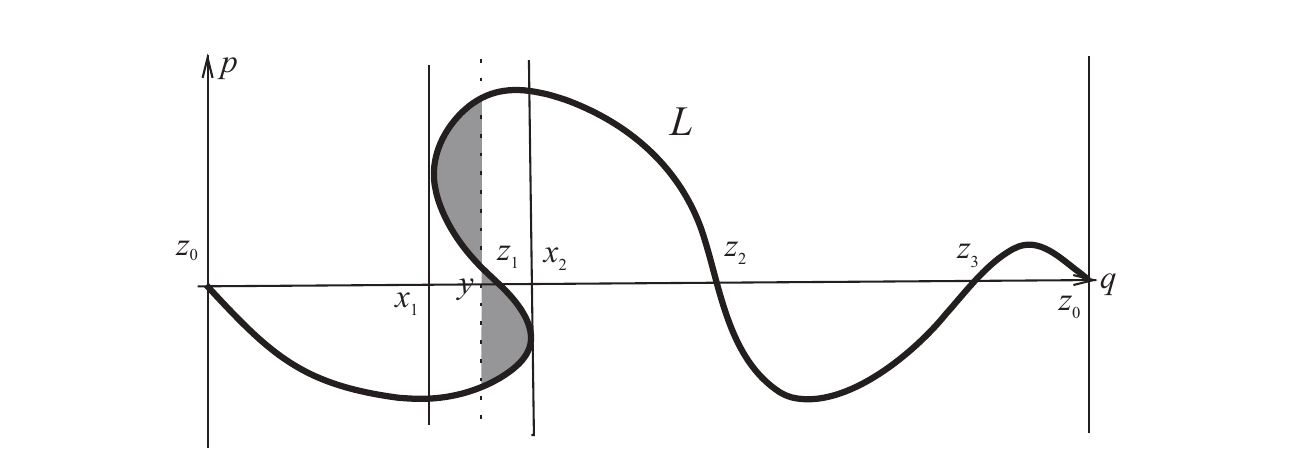
\includegraphics[width=0.9\textwidth]{chapters/ch12-cotangent-floer/figures/ch12-figure-12-1.png}
  \caption{\termMultisectionLagrangian{} $L$。}
  \label{fig:multisection-lagrangian}
\end{figure}

为了说明 $f_H$ 的含义，下面给出 $N=S^1$ 时的一个例子。

\begin{example}
\label{ex:wave-front-circle-multisection}
考虑\cref{fig:multisection-lagrangian}所示的拉格朗日子流形 $L\subset T^*S^1$。这里用 $z_i$ 表示 $L$ 与零截面的交点，用 $x_i$ 表示\termCaustic{}，并用 $y$ 表示图中两个阴影区域面积相等的点。相应的波前不难画成\cref{fig:wave-front-basic-phase}所示。

\begin{figure}[htbp]
  \centering
  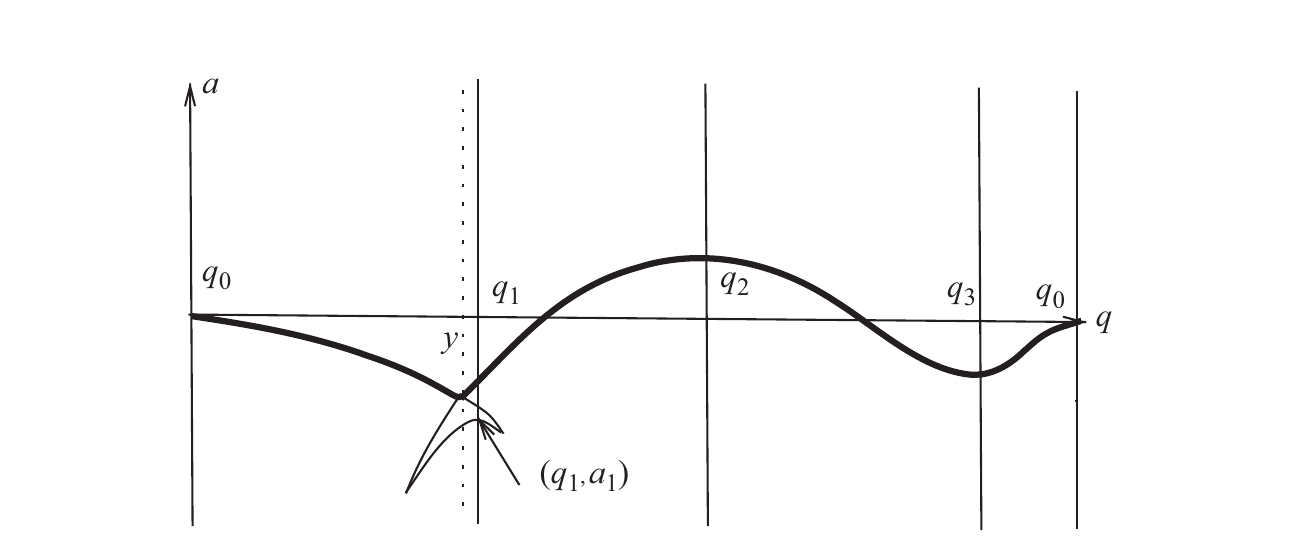
\includegraphics[width=0.88\textwidth]{chapters/ch12-cotangent-floer/figures/ch12-figure-12-2.png}
  \caption{$L$ 的\termWaveFront{}与 $f_H$ 的图。}
  \label{fig:wave-front-basic-phase}
\end{figure}

注意，$z_i$ 对应于作用量泛函的临界点，$x_i$ 对应于波前的\termCuspPoint{}，而 $y$ 对应于波前的两个不同分支相交之点。利用 $H\mapsto L$ 时基本相位函数 $f_H$ 的连续性，不难看出 $f_H$ 的图正是\cref{fig:wave-front-basic-phase}中的粗线。我们还要指出，数值
\[
  \min_{q\in N}f_H(q)
\]
\emph{并不是} $\mathcal A_H$ 的临界值，而是与波前交叉相伴的一个值。\footnote{译者注：原书末句把本节的 $f_H$ 突然写成此前未定义的 $F^H$；译文改回 $f_H$。}
\end{example}

